\section*{Supplementary material}
\paragraph{Outline.} In Sec.~\ref{sec:proofs} we provide the proofs of the propositions and theorems given in the main paper. In Sec.~\ref{sec:discrete} we consider the discretized problems and obtain similar results. In Sec.~\ref{sec:other-pptys} we show additional properties of the problem considered. Finally in Sec.~\ref{sec:addexp} we give more illustrations of barycenters and show the effect of the regularization on the accuracy of our proposed algorithm. 


\section{Proofs}
\label{sec:proofs}
\subsection{Notations}


Let $\mathcal{Z}$ be a Polish space, we denote $\mathcal{M}(\mathcal{Z})$ the set of Radon measures on $\mathcal{Z}$ endowed with total variation norm: $\lVert\mu\rVert_{\TV}=\mu_+(\mathcal{Z})+\mu_-(\mathcal{Z})$ with $(\mu_+,\mu_-)$ is the Dunford decomposition of the signed measure $\mu$. We call $\mathcal{M}_+(\mathcal{Z})$ the sets of positive Radon measures, and  $\mathcal{M}^1_+(\mathcal{Z})$ the set of probability measures. We denote $\mathcal{C}^b(\mathcal{Z})$ the vector space of bounded continuous functions on $\mathcal{Z}$ endowed with $\lVert\cdot \rVert_\infty$ norm. We recall the \textit{Riesz-Markov theorem}: if $\mathcal{Z}$ is compact, $\mathcal{M}(\mathcal{Z})$ is the topological dual of $\mathcal{C}^b(\mathcal{Z})$. Let $\mathcal{X}$ and $\mathcal{Y}$ be two Polish spaces. It is immediate  that \textit{$\mathcal{X}\times\mathcal{Y}$ is a Polish space}.  We denote $\Pi_1:(x,y)\in\mathcal{X}\times\mathcal{Y}\mapsto x$ and $\Pi_2:(x,y)\in\mathcal{X}\times\mathcal{Y}\mapsto y$ respectively the projections on $\mathcal{X}$ and  $\mathcal{Y}$, which are continuous applications. For an application $g$ and a measure $\mu$, we denote $g_\sharp\mu$ the pushforward measure of $\mu$ by $g$. For $f:\mathcal{X}\rightarrow\mathbb{R}$ and $g:\mathcal{Y}\rightarrow\mathbb{R}$, we denote $f\oplus g:(x,y)\in\mathcal{X}\times\mathcal{Y}\mapsto f(x)+g(y)$ the tensor sum of $f$ and $g$. For  $\mathcal{X}$ and $\mathcal{Y}$ two Polish spaces, we denote $\text{LSC}(\mathcal{X}\times\mathcal{Y})$ the space of lower semi-continuous functions on $\mathcal{X}\times\mathcal{Y}$.


\subsection{Proof of Theorem~\ref{thm:duality-GOT}}
\label{prv:duality-GOT}
% \begin{thm*}[Strong Duality]
% Let $\mathcal{X}$ and $\mathcal{Y}$ be Polish spaces. Let $\mathbf{c}=(c_i)_{1\leq i\leq N}$ be a family of nonnegative lower semi-continuous costs. Then \emph{strong duality holds} that is for all $\mu\in\mathcal{M}_{+}^{1}(\mathcal{X})$ and $\nu\in\mathcal{M}_{+}^{1}(\mathcal{Y})$ 
% \begin{align*}
%   \MOT_{\mathbf{c}}(\mu,\nu) =\sup_{\lambda\in\Delta_N} \sup\limits_{(f,g)\in\mathcal{F}_{\mathbf{c}}^{\lambda}}\int_{x\in\mathcal{X}} f(x)d\mu(x)+ \int_{y\in\mathcal{Y}} g(y)d\nu(y)
% \end{align*}
% and the infimum of the primal problem~(\ref{eq-primal}) is attained.
% \end{thm*}

To prove this theorem, we use an equivalent form of the problem, presented in Section~\ref{sec:other-pptys}. 
%Indeed, the proof we present allows extension to lower semi-continuous costs.
\begin{prv*}
In Proposition~\ref{prop:duality-max}, we  proved that 
$$\MOT_{\mathbf{c}}(\mu,\nu) =\sup_{\lambda\in\Delta^+_N} \sup\limits_{(f,g)\in\mathcal{F}_{\mathbf{c}}^{\lambda}}\int_{x\in\mathcal{X}} f(x)d\mu(x)+ \int_{y\in\mathcal{Y}} g(y)d\nu(y).$$ 
Let show that we can extend the search space for $\lambda$ to $\Delta_N$. Denote by $$\mathcal{F}_{\mathbf{c}}:=\left\{(f,g)\in\mathcal{C}^b(\mathcal{X})\times \mathcal{C}^b(\mathcal{Y})~\mathrm{s.t.}~\exists\lambda\in\Delta_N,~\forall i,~f\oplus g\leq \lambda_i c_i\right\}$$
and 
$$\mathcal{F}_{\mathbf{c}}^+:=\left\{(f,g)\in\mathcal{C}^b(\mathcal{X})\times \mathcal{C}^b(\mathcal{Y})~\mathrm{s.t.}~\exists\lambda\in\Delta^+_N,~\forall i,~f\oplus g\leq \lambda_i c_i\right\}.$$
Moreover by denoting 
$$\mathcal{G}_{\mathbf{c}}:=\left\{(f,g)\in\mathcal{C}^b(\mathcal{X})\times \mathcal{C}^b(\mathcal{Y})~\mathrm{s.t.}~\exists\lambda\in\Delta_N\setminus\Delta_N^{+} ,~\forall i,~f\oplus g\leq \lambda_i c_i\right\},$$
we have therefore that $\mathcal{F}_{\mathbf{c}}= \mathcal{F}_{\mathbf{c}}^+\sqcup \mathcal{G}_{\mathbf{c}}$
and it is clear
\begin{align*}
   \sup\limits_{(f,g)\in\mathcal{F}_{\mathbf{c}}^+}\int_{x\in\mathcal{X}} f(x)d\mu(x)+ \int_{y\in\mathcal{Y}} g(y)d\nu(y)\leq  \sup\limits_{(f,g)\in\mathcal{F}_{\mathbf{c}}}\int_{x\in\mathcal{X}} f(x)d\mu(x)+ \int_{y\in\mathcal{Y}} g(y)d\nu(y)
\end{align*}
Let us now consider $(f,g)\in \mathcal{G}_{\mathbf{c}}$. Therefore  there exists a $\lambda\in\Delta_N$ and $k$ such that $\lambda_k< 0$, so that $f \oplus g\leq \lambda_k c_k$, which by positivity of the cost functions leads that 
\begin{align}
    \sup\limits_{(f,g)\in\mathcal{G}_{\mathbf{c}}}\int_{x\in\mathcal{X}} f(x)d\mu(x)+ \int_{y\in\mathcal{Y}} g(y)d\nu(y)\leq 0
\end{align}
But thanks to Proposition \ref{prop:duality-max}, we have that
$$\MOT_{\mathbf{c}}(\mu,\nu)= \sup\limits_{(f,g)\in\mathcal{F}_{\mathbf{c}}^+}\int_{x\in\mathcal{X}} f(x)d\mu(x)+ \int_{y\in\mathcal{Y}} g(y)d\nu(y).$$
But by definition, $\MOT_{\mathbf{c}}(\mu,\nu)$ is non-negative, therefore we have that 
$$ \sup\limits_{(f,g)\in\mathcal{G}_{\mathbf{c}}}\int_{x\in\mathcal{X}} f(x)d\mu(x)+ \int_{y\in\mathcal{Y}} g(y)d\nu(y)\leq  \sup\limits_{(f,g)\in\mathcal{F}_{\mathbf{c}}^+}\int_{x\in\mathcal{X}} f(x)d\mu(x)+ \int_{y\in\mathcal{Y}} g(y)d\nu(y)$$
and the result follows.




% But thanks to Proposition \ref{prop:duality-max}, we have that
% $$\MOT_{\mathbf{c}}(\mu,\nu)=
% \sup\limits_{(f,g)\in\mathcal{F}_{\mathbf{c}}^+}\int_{x\in\mathcal{X}} f(x)d\mu(x)+ \int_{y\in\mathcal{Y}} g(y)d\nu(y).$$
% But by definition, $\MOT_{\mathbf{c}}(\mu,\nu)$ is non-negative, therefore we have that 
% $$\sup\limits_{(f,g)\in\mathcal{F}_{\mathbf{c}}^+}\int_{x\in\mathcal{X}} f(x)d\mu(x)+ \int_{y\in\mathcal{Y}} g(y)d\nu(y)=0$$
% which is a contradiction.



\end{prv*}


% \begin{lemma}
% \label{lem:compact-weak}
% Let $\mathcal{X}$ and $\mathcal{Y}$ be Polish spaces, and $\mu$ and $\nu$ two probability measures respectively on  $\mathcal{X}$ and $\mathcal{Y}$. Then $\Gamma^N_{\mu,\nu}$  is sequentially compact for the weak topology induced by $\Vert \gamma \Vert = \max\limits_{i=1,..,N} \Vert \gamma_i\Vert_{\TV}$. 
% \end{lemma}


% \begin{prv*}
% Let $(\gamma^n)_{n\geq 0}$ a sequence in $\Gamma^N_{\mu,\nu}$, and let us denote for all $n\geq 0$, $\gamma^n=(\gamma^n_i)_{i=1}^N$. We first remarks that for all $i\in\{1,...,N\}$ and $n\geq 0$, $\Vert \gamma_i^n\Vert_{\TV}\leq 1$ therefore for all $i\in\{1,...,N\}$, $(\gamma^n_i)_{n\geq 0}$ is uniformly bounded. Moreover as $\{\mu\}$ and $\{\nu\}$ are tight, for any $\delta>0$, there exists $K\subset \mathcal{X} $ and $L\subset \mathcal{Y}$ compact such that 
% \begin{align}
%     \mu(K^c)\leq \frac{\delta}{2} \text{\quad and\quad }  \nu(L^c)\leq \frac{\delta}{2}.
% \end{align}
% Therefore, we obtain that for any for all $i\in\{1,...,N\}$,
% \begin{align}
%     \gamma_i^n(K^c\times L^c)&\leq \sum_{k=1}^N \gamma_k^n(K^c\times L^c)\\
%     &\leq  \sum_{k=1}^N \gamma_k^n(K^c\times\mathcal{Y})+\gamma_k^n(\mathcal{X}\times L^c)\\
%     &\leq  \mu(K^c) + \nu(L^c) = \delta.
% \end{align}
% Therefore, for all $i\in\{1,...,N\}$,  $(\gamma_i^n)_{n\geq 0}$ is tight and uniformly bounded and Prokhorov's theorem~\citep[Theorem A.3.15]{dupuis2011weak} guarantees for all $i\in\{1,...,N\}$,  $(\gamma_i^n)_{n\geq 0}$ admits a weakly convergent subsequence. By extracting a common convergent subsequence, we obtain that $(\gamma^n)_{n\geq 0}$ admits a weakly convergent subsequence. By continuity of the projection, the limit also lives in $\Gamma
% ^N_{\mu,\nu}$ and the result follows.
% \end{prv*}
% \begin{lemma}
% \label{lem:rockafellar-gene}
% Let $V$ be a normed vector space and $V^*$ its topological dual. Let $V_1,...,V_N$ be convex functions and lower semi-continuous on $V$ and $E$ a convex function on $V$. Let $V^*_1,...V^*_N,E^*$ be the Fenchel-Legendre transforms of $V_1,...V_N,E$. Assume there exists $z_0\in V$ such that for all $i$, $V_i(z_0)<\infty$, $E(z_0)<\infty$, and for all $i$, $V_i$ is continuous at $z_0$. Then:
% \begin{align*}
% \inf_{u\in V} \sum_i V_i(u) + E(u) = \sup\limits_{\substack{\gamma_1...,\gamma_N,\gamma\in V^*\\\sum_i \gamma_i = \gamma}}-\sum_i V^*_i(-\gamma_i)-E^*(\gamma)
% \end{align*}
% \end{lemma}
% \begin{prv*}
% This Lemma is an immediate application of Rockafellar-Fenchel duality theorem~\citep[Theorem 1.12]{brezis2010functional} and of Fenchel-Moreau theorem~\citep[Theorem 1.11]{brezis2010functional}. 
% Indeed, $V = \sum\limits_{i=1}^N V_i(u)$ is a convex function, lower semi-continuous and its Legendre-Fenchel transform is given by:
% \begin{align}
%     V^{*}(\gamma^*)=\inf_{\sum\limits_{i=1}^N \gamma_{i}^*=\gamma^*}\sum_{i=1}^N V_i^{*}(\gamma_{i}^*).
% \end{align}
% \end{prv*}


% % \begin{lemma}
% % \label{lem:mot-max}
% % \label{lem:technical-lemma-primal}
% % Let $\mathcal{X}$ and $\mathcal{Y}$ be Polish spaces. Let $\mathbf{c}=(c_i)_{1\leq i\leq N}$ be a family of nonnegative lower semi-continuous costs on $\mathcal{X}\times \mathcal{Y}$, then for $\mu\in\mathcal{M}^1_+(\mathcal{X})$ and  $\nu\in\mathcal{M}^1_+(\mathcal{Y})$, we have
% % \begin{align}
% % \label{eq:max-mot}
% % \MOT_{\mathbf{c}}(\mu,\nu)= \inf_{\gamma\in\Gamma_{\mu,\nu}^N} \max_i\int_{\mathcal{X}\times\mathcal{Y}}c_i(x,y)d\gamma_i(x,y)
% % \end{align}
% % \end{lemma}

% % \begin{prv*}
% % It is clear that $\MOT_{\mathbf{c}}(\mu,\nu)\leq \inf_{\gamma\in\Gamma_{\mu,\nu}^N} \max_i\int_{\mathcal{X}\times\mathcal{Y}}c_i(x,y)d\gamma_i(x,y)$. The infimum is attained for both problem thanks to weak compactness of $\Gamma_{\mu,\nu}^N$ (Lemma~\ref{lem:compact-weak}) and Stone Weierstrass Lemma. Let $\gamma^*$ be the optimum for $\inf_{\gamma\in\Gamma_{\mu,\nu}^N} \max_i\int_{\mathcal{X}\times\mathcal{Y}}c_i(x,y)d\gamma_i(x,y)$. 

% % Assume there exists $i,j$ such that $\int c_i d\gamma_i>\int c_j d\gamma_j$
% % \end{prv*}


% \begin{lemma}
% \label{lem:technical-lemma-primal}
% Let $\mathcal{X}$ and $\mathcal{Y}$ be Polish spaces. Let $\mathbf{c}=(c_i)_{1\leq i\leq N}$ be a family of nonnegative lower semi-continuous costs on $\mathcal{X}\times \mathcal{Y}$, then for $\mu\in\mathcal{M}^1_+(\mathcal{X})$ and  $\nu\in\mathcal{M}^1_+(\mathcal{Y})$, we have
% \begin{align}
% \label{eq:supinf}
% \MOT_{\mathbf{c}}(\mu,\nu)= \sup_{\lambda\in\Delta_N}\inf_{\gamma\in\Gamma_{\mu,\nu}^N} \sum_{i=1}^N\lambda_i\int_{\mathcal{X}\times\mathcal{Y}}c_i(x,y)d\gamma_i(x,y)
% \end{align}
% and the infimum is attained.
% % and both the infimum and the supremum are attained. Moreover, if $\gamma^*$ be an optimum for~\eqref{eq-primal} and $\lambda^*$ an optimum for~\eqref{eq:supinf}, then $(\lambda^*,\gamma^*)$ is a saddle point for the minmax problem.
% \end{lemma}

% \begin{prv*}
% Taking for granted that a minmax principle can be invoked, we have
% \begin{align*}
%     \sup_{\lambda\in\Delta_N}\inf_{\gamma\in\Gamma_{\mu,\nu}^N} \sum_{i=1}^N\lambda_i\int_{\mathcal{X}\times\mathcal{Y}}c_i(x,y)d\gamma_i(x,y) &= \inf_{\gamma\in\Gamma_{\mu,\nu}^N}\sup_{\lambda\in \Delta_N} \sum_{i=1}^N\lambda_i\int_{\mathcal{X}\times\mathcal{Y}}c_i(x,y)d\gamma_i(x,y)\\
%     % &=\inf_{\gamma\in\Gamma_{\mu,\nu}^N}\max_{i} \int_{\mathcal{X}\times\mathcal{Y}}c_i(x,y)d\gamma_i(x,y)\\
%     &=\MOT_{\mathbf{c}}(\mu,\nu)
% \end{align*}
% But thanks to Lemma \ref{lem:compact-weak}, we have that $\Gamma_{\mu,\nu}^N$ is compact for the weak topology. And $\Delta_N$ is convex. Moreover the objective function $f:(\lambda,\gamma)\in\Delta_N\times\Gamma^N_{\mu,\nu} \mapsto \sum_{i=1}^N\lambda_i \int_{\mathcal{X}\times \mathcal{Y}} c^n_id\gamma_i$ is bilinear, hence convex and concave  in its variables, and continuous with respect to $\lambda$. Moreover, let $(c^n_i)_n$ be non-decreasing sequences of non-negative bounded cost functions such that $c_i=\sup_n c^n_i$. By monotone convergence, we get $f(\lambda,\gamma) = \sup_n \sum_i\lambda_i \int c^n_i d\gamma_i$, $f(\lambda,.)$. So $f$ the supremum of continuous functions, then $f$ is lower semi-continuous with respect to $\gamma$, therefore Sion's minimax theorem
% ~\citep{sion1958} holds.
% %Moreover $\lambda\in\Delta_N \rightarrow \min_{\gamma\in\Gamma_{P,Q}^N} f(\lambda,\gamma)$ is upper semi continuous as being a infimum of linear (hence continuous) functions. Then then by compacity of $\Delta_N$ we can apply the Stone-Weierstass Theorem~\citep[Theorem 5.8]{rudin1991functional} which conclude the existence of minimum and supremum.

% % Let $\gamma^*$ be the optimum for~\eqref{eq-primal} and $\lambda^*$ the optimum for~\eqref{eq:supinf}. Since $f:(\lambda,\gamma)\mapsto\sum_{i=1}^N\lambda_i\int_{\mathcal{X}\times\mathcal{Y}}c_i(x,y)d\gamma_i(x,y)$ is linear in both variables, the optimal value of~\eqref{eq-primal} and~\eqref{eq:supinf} coincide at $f(\lambda^*,\gamma^*)$. Following the standard results from convex analysis~\citep[Lemma 36.2, Corollary  37.6.2]{rockafellar1970convex}, $(\lambda^*,\gamma^*)$ is a saddle point for the minmax problem.
% \end{prv*}

% \begin{thm*}[Strong Duality]
% Let $\mathcal{X}$ and $\mathcal{Y}$ be Polish spaces. Let $\mathbf{c}=(c_i)_{1\leq i\leq N}$ be a family of nonnegative lower semi-continuous costs. Then \emph{strong duality holds} that is for all $\mu\in\mathcal{M}_{+}^{1}(\mathcal{X})$ and $\nu\in\mathcal{M}_{+}^{1}(\mathcal{Y})$ 
% \begin{align*}
%   \MOT_{\mathbf{c}}(\mu,\nu) =\sup_{\lambda\in\Delta_N} \sup\limits_{(f,g)\in\mathcal{F}_{\mathbf{c}}^{\lambda}}\int_{x\in\mathcal{X}} f(x)d\mu(x)+ \int_{y\in\mathcal{Y}} g(y)d\nu(y)
% \end{align*}
% and the infimum of the primal problem~(\ref{eq-primal}) is attained.
% \end{thm*}
% \begin{prv*}
% Let $\mathcal{X}$ and $\mathcal{Y}$ be two Polish spaces. For all $i\in \{1,..,N\}$, we define $c_i:\mathcal{X}\times\mathcal{Y}\rightarrow \mathbb{R}^+$ a cost function. The proof follows the exact same steps as those in the proof of~\citep[Theorem 1.3]{villani2003topics}. First we suppose that $\mathcal{X}$ and $\mathcal{Y}$ are compact and that for all $i$, $c_i$ is continuous, then we show that it can be extended to $X$ and $Y$ non compact and finally to $c_i$ only lower semi continuous.

% \medskip
% First, let assume $\mathcal{X}$ and $\mathcal{Y}$ are compact and that for all $i$, $c_i$ is continuous. Let fix $\lambda \in\Delta_N$. We recall the topological dual of the space of bounded continuous functions $\mathcal{C}^b(\mathcal{X}\times\mathcal{Y})$ endowed with $\lVert.\rVert_\infty$ norm, is the space of Radon measures $\mathcal{M}(\mathcal{X}\times\mathcal{Y})$ endowed with total variation norm. We define, for $u\in \mathcal{C}^b(\mathcal{X}\times\mathcal{Y})$:
% \begin{align*}
% V^\lambda_i(u) =
% \left\{\begin{matrix} 0 &\quad\text{if}\quad& u\geq -\lambda_i c_i\\
% +\infty &\quad\text{else}\quad&\end{matrix}\right.
% \end{align*}
% and:
% \begin{align*}
% E(u)=\left\{\begin{matrix} \int fd\mu+\int gd\nu &\quad\text{if}\quad& \exists (f,g)\in \mathcal{C}^b(\mathcal{X})\times \mathcal{C}^b(\mathcal{Y}),~ u = f+g\\
% +\infty &\quad\text{else}\quad&\end{matrix}\right.
% \end{align*}
% One can show that for all $i$, $V^\lambda_i$ is convex and lower semi-continuous (as the sublevel sets are closed) and $E^\lambda$ is convex. More over for all $i$, these functions continuous in $u_0\equiv 1$ the hypothesis of Lemma~\ref{lem:rockafellar-gene} are satisfied.


% Let now compute the Fenchel-Legendre transform of these function.  Let $\gamma\in \mathcal{M}(\mathcal{X}\times\mathcal{Y})$ :

% \begin{align*}
% V^{\lambda*}_i(-\gamma) &= \sup_{u\in \mathcal{C}^b(\mathcal{X}\times\mathcal{Y})}\left\{-\int ud\gamma;\quad u\geq-\lambda_i c_i\right\}
% \\
% & = \left\{\begin{matrix}\int \lambda_i c_i d\gamma &\quad\text{if} \quad& \gamma\in\mathcal{M}_+(\mathcal{X}\times\mathcal{Y}) \\
% +\infty &\quad\text{otherwise}\quad& \end{matrix}\right.
% \end{align*}

% On  the other hand:
% \begin{align*}
% E^{\lambda*}(\gamma)=\left\{\begin{matrix} 0 &\quad\text{if}\quad& \forall (f,g)\in \mathcal{C}^b(\mathcal{X})\times \mathcal{C}^b(\mathcal{Y}),~ \int fd\mu+\int gd\nu  = \int (f+g)d\gamma\\
% +\infty &\quad\text{else}\quad&\end{matrix}\right.
% \end{align*}
% This dual function is finite and equals $0$ if and only if that the marginals of the dual variable $\gamma$ are $\mu$ and $\nu$. 

% Applying Lemma~\ref{lem:rockafellar-gene}, we get:
% \begin{align*}
% \inf_{u\in \mathcal{C}^b(\mathcal{X}\times\mathcal{Y})} \sum_i V^{\lambda}_i(u)+E(u) = \sup\limits_{\substack{\gamma_1,...,\gamma_N,\gamma\in \mathcal{M}(\mathcal{X}\times\mathcal{Y})\\\sum\gamma_i=\gamma}}\sum -V^{\lambda*}_i(\gamma_i)-E^{\lambda*}(-\gamma)
% \end{align*}



% Hence, we  have shown that, when $\mathcal{X}$ and $\mathcal{Y}$ are compact sets, and  the costs $(c_i)_i$ are continuous:
% \begin{align*}
% \sup\limits_{(f,g)\in\mathcal{F}^\lambda_\mathbf{c}}\int fd\mu+\int gd\nu = \inf\limits_{\gamma\in\Gamma^N_{\mu,\nu}}\sum_i\lambda_i \int c_id\gamma_i
% \end{align*}



% % We now apply Lemma CITE to get the strong duality:
% % \begin{align*}
% %     WRITE EQUATION
% % \end{align*}
% % when $\mathbf{c}$ is a family of continuous and sets $\mathcal{X}$ and $\mathcal{Y}$ are compact. 
% % Now we need  to prove that we can intervert the supremum over $\lambda\in U:=\{(\lambda_i)_{i\in\Theta}\text{ s.t. }\forall i,~\lambda_i\geq 0\text{ and }\sum_i\lambda_i=1\} $  and the infimum over $\gamma\in V:=\Pi_{P,Q}$.   Let call $f(\lambda,\gamma) = \sum_i\lambda_i \int c_id\gamma_i$. It is clear that $U$ is compact convex, that $V$ is convex and compact for weak topology, and  $f$ is bilinear and continuous in both variables. We can apply Sion's theorem ADD REF and then:
% % \begin{align*}
% % \sup\limits_{\substack{\lambda\in\mathbb{R}^K\\\lambda\geq 0\\\sum_i\lambda_i=1}}\inf\limits_{\substack{\sub(\gamma_i)_{i\in\Theta}\in\mathcal{M}_+(\mathcal{X}\times\mathcal{Y})^K\\ \Pi_1\#\sum_i\gamma_i = P\\
% % \Pi_2\#\sum_i\gamma_i = Q}}\sum_i\lambda_i \int c_id\gamma_i &=\inf\limits_{\substack{\sub(\gamma_i)_{i\in\Theta}\in\mathcal{M}^+(\mathcal{X}\times\mathcal{Y})^K\\ \Pi_1\#\sum_i\gamma_i = P\\
% % \Pi_2\#\sum_i\gamma_i = Q}}\sup\limits_{\substack{\lambda\in\mathbb{R}^K\\\lambda\geq 0\\\sum_i\lambda_i=1}} \sum_i\lambda_i \int c_id\gamma_i\\
% % &=\inf\limits_{\substack{\sub(\gamma_i)_{i\in\Theta}\in\mathcal{M}^+(\mathcal{X}\times\mathcal{Y})^K\\ \Pi_1\#\sum_i\gamma_i = P\\
% % \Pi_2\#\sum_i\gamma_i = Q}}\max_i \int c_id\gamma_i
% % \end{align*}

% \medskip

% Let now prove  the result holds when the spaces $\mathcal{X}$ and $\mathcal{Y}$ are not compact. We still suppose that for all $i$, $c_i$ is uniformly continuous and bounded. We denote $\Vert\mathbf{c}\rVert_\infty := \sup_i \sup_{(x,y)\in\mathcal{X}\times\mathcal{Y}} c_i(x,y)$.  Let define $I^\lambda(\gamma):=\sum_i\lambda_i\int_{\mathcal{X}\times\mathcal{Y}}c_id\gamma_i$

% Let $\gamma^*\in \Gamma^N_{\mu,\nu}$ such that $I^\lambda(\gamma^*) =\min_{\gamma\in\Gamma^N_{\mu,\nu}}I^\lambda(\gamma)$.  The existence of the minimum comes from the lower-semi continuity of $I^\lambda$ and  the compacity of $\Gamma^N_{\mu,\nu}$ for weak topology.

% Let fix $\delta\in (0,1)$. $\mathcal{X}$ and $\mathcal{Y}$ are Polish spaces then $\exists  \mathcal{X}_0\subset \mathcal{X},  \mathcal{Y}_0\subset \mathcal{Y}$ compacts such that $\mu(\mathcal{X}_0^c) \leq  \delta$ and $\mu(\mathcal{Y}_0^c) \leq  \delta$.  It follows that $\forall i$, $\gamma^*_i((\mathcal{X}_0\times\mathcal{Y}_0)^c)\leq 2\delta$. Let define $\gamma^{*0}$ such that for all $i$, $\gamma^{*0}_{i}=\frac{\mathbf{1}_{\mathcal{X}_0\times\mathcal{Y}_0}}{\sum_i\gamma_i
% ^*(\mathcal{X}_0\times\mathcal{Y}_0)}\gamma^*_i$. We define $\mu_0 = \Pi_{1\sharp}\sum_i\gamma_{i}^{*0}$ and  $\nu_0 = \Pi_{2\sharp}\sum_i\gamma_{i}^{*0}$. We then naturally define $\Gamma^{N}_{0,\mu_0,\nu_0} :=\left\{(\gamma_i)_{1\leq i\leq N}\in \mathcal{M}_+(\mathcal{X}_0\times \mathcal{Y}_0)^N\text{ s.t. } \Pi_{1\sharp}\sum_i\gamma_i=\mu_0 \text{ and } \Pi_{2\sharp}\sum_i\gamma_i=\nu_0\right\}$ and $I^\lambda_0(\gamma_0) := \sum_i\lambda_i\int_{\mathcal{X}_0\times\mathcal{Y}_0}c_id\gamma_{0,i}$ for $\gamma_0\in\Gamma^{N}_{0,\mu_0,\nu_0}$. 

% Let $\tilde{\gamma}_0$ verifying  $I^\lambda_0(\tilde{\gamma}_0) = \min_{\gamma_0\in\Pi^N_{0,\mu_0,\nu_0}}I^\lambda_0(\gamma_0)$. Let $\tilde{\gamma} = \left(\sum_i\gamma_i^*(\mathcal{X}_0\times\mathcal{Y}_0)\right)\tilde{\gamma}_0+\mathbf{1}_{(\mathcal{X}_0\times\mathcal{Y}_0)^c}\gamma^*\in \Gamma^N_{\mu,\nu}$. Then we get 
% \begin{align*}
% I^\lambda(\tilde{\gamma})\leq \min_{\gamma_0\in\Gamma^N_{0,\mu_0,\nu_0}}I^\lambda_0(\gamma_0)+2\sum|\lambda_i|\lVert \mathbf{c}\rVert_\infty\delta
% \end{align*}

% We have already proved that:

% \begin{align*}
% \sup\limits_{(f,g)\in\mathcal{F}^\lambda_{0,\mathbf{c}}}J_0^\lambda(f,g) = \inf\limits_{\gamma_0\in\Gamma^N_{0,\mu_0,\nu_0}}I_0^\lambda(\gamma_0)
% \end{align*}

% with $J_0^\lambda(f,g) = \int fd\mu_0+\int gd\nu_0$ and $\mathcal{F}^\lambda_{0,\mathbf{c}}$ is the set of $(f,g)\in\mathcal{C}^b(\mathcal{X}_0)\times \mathcal{C}^b(\mathcal{Y}_0)$ satisfying, for every $i$, $f\oplus g\leq\min_i\lambda_i c_i$. Let $(\tilde{f}_0,\tilde{g}_0)\in \mathcal{F}^\lambda_\mathbf{0,c}$ such that :
% \begin{align*}
%     J_0^\lambda(\tilde{f}_0,\tilde{g}_0)\geq \sup\limits_{(f,g)\in\mathcal{F}^\lambda_{0,\mathbf{c}}}J_0^\lambda(f,g)-\delta
% \end{align*}
% Since $J_0^\lambda(0,0)=0$, we get $\sup J_0^\lambda\geq 0$ and then,  $J_0^\lambda(\tilde{f}_0,\tilde{g}_0)\geq \delta\geq-1$. For every $\gamma_0 \in \Gamma^N_{0,\mu_0,\nu_0}$:

% \begin{align*}
% J_0^\lambda(\tilde{f}_0,\tilde{g}_0) = \int (\tilde{f}_0(x)+\tilde{g}_0(y))d\gamma_0(x,y)
% \end{align*}
% then we have the existence of $(x_0,y_0)\in\mathcal{X}_0\times\mathcal{Y}_0$ such that : $\tilde{f}_0(x_0)+\tilde{g}_0(y_0)\geq -1$. If we replace $(\tilde{f}_0,\tilde{g}_0)$ by $(\tilde{f}_0-s,\tilde{g}_0+s)$ for an accurate $s$, we get that: $\tilde{f}_0(x_0)\geq \frac12$
% and $\tilde{g}_0(y_0)\geq \frac12$, and then $\forall(x,y)\in\mathcal{X}_0\times\mathcal{Y}_0$:
% \begin{align*}
%     \tilde{f}_0(x)\leq c'(x,y_0)-\tilde{g}_0(y_0)\leq c'(x,y_0)+\frac12\\
%     \tilde{g}_0(y)\leq c'(x_0,y)-\tilde{f}_0(x_0)\leq c'(x_0,y)+\frac12
% \end{align*}
% where $c':=\min_i\lambda_ic_i$.  Let define $\bar{f}_0(x) = \inf_{y\in\mathcal{Y}_0}c'(x,y)-\tilde{g}_0(y)$ for $x\in\mathcal{X}$.  Then $\tilde{f}_0\leq \bar{f}_0$ on $\mathcal{X}_0$. We then get $J_0^\lambda(\bar{f}_0,\tilde{g}_0)\geq J_0^\lambda(\tilde{f}_0,\tilde{g}_0)$ and $\bar{f}_0\leq c'(.,y_0)+\frac12$ on $\mathcal{X}$. Let define $\bar{g}_0(y)= \inf_{x\in\mathcal{X}}c'(x,y)-\bar{f}_0(y)$. By construction $(f_0,g_0)\in \mathcal{F}
% ^\lambda_\mathbf{c}$ since the costs are uniformly continuous and bounded and $J_0^\lambda(\bar{f}_0,\bar{g}_0)\geq J_0^\lambda(\bar{f}_0,\tilde{g}_0)\geq J_0^\lambda(\tilde{f}_0,\tilde{g}_0)$. We also have  $\bar{g}_0\geq c'(x_0,.)+\frac12$ on $\mathcal{Y}$. Then we have in particular: $\bar{g}_0\geq -\lVert\mathbf{c}\rVert_\infty-\frac12$ on $\mathcal{X}$ and $\bar{f}_0\geq -\lVert\mathbf{c}\rVert_\infty-\frac12$ on $\mathcal{Y}$. Finally:

% \begin{align*}
% J^\lambda(\bar{f}_0,\bar{g}_0)&:=\int_{\mathcal{X}_0}\bar{f}d\mu_0+\int_{\mathcal{Y}_0}\bar{g}_0d\nu\\
% &=\sum_i\gamma_i^*(\mathcal{X}_0\times\mathcal{Y}_0)\int_{\mathcal{X}_0\times\mathcal{Y}_0}(\bar{f}_0(x)+\bar{g}_0(y))d\left(\sum_i\gamma^{*0}_i(x,y)\right)\\
% &+\int_{(\mathcal{X}_0\times\mathcal{Y}_0)^c}\bar{f}_0(x)+\bar{g}_0(y)d\left(\sum_i\gamma^{*}_i(x,y)\right)\\
% &\geq (1-2\delta)\left(\int_{\mathcal{X}_0}\bar{f}_0d\mu_0+\int_{\mathcal{Y}_0}\bar{g}_0d\nu_0\right)-(2\lVert\mathbf{c}\rVert_\infty+1)\sum_i\gamma^*((\mathcal{X}_0\times\mathcal{Y}_0)^c)\\
% &\geq (1-2\delta)J_0^\lambda(\bar{f}_0,\bar{g}_0)-2\sum |\lambda_i|(2\lVert\mathbf{c}\rVert_\infty+1)\delta\\
% &\geq (1-2\delta)J_0^\lambda(\tilde{f}_0,\tilde{g}_0)-2\sum |\lambda_i|(2\lVert\mathbf{c}\rVert_\infty+1)\delta\\
% &\geq (1-2\delta)(\inf I^\lambda_0-\delta)-2\sum |\lambda_i|(2\lVert\mathbf{c}\rVert_\infty+1)\delta\\
% &\geq  (1-2\delta)(\inf I^\lambda-(2\sum |\lambda_i|\lVert\mathbf{c}\rVert_\infty+1)\delta)-2\sum |\lambda_i|(2\lVert\mathbf{c}\rVert_\infty+1)\delta
% \end{align*}

% This being true for arbitrary small $\delta$, we get $\sup J^\lambda\geq\inf I^\lambda$. The other sens is always true then:
% \begin{align*}
% \sup\limits_{(f,g)\in\mathcal{F}^\lambda_\mathbf{c}}\int fd\mu+\int gd\nu = \inf\limits_{\gamma\in\Gamma^N_{\mu,\nu}}\sum_i\lambda_i \int c_id\gamma_i
% \end{align*}

% for $c_i$ uniformly continuous and $\mathcal{X}$ and $\mathcal{Y}$ non necessarily compact.

% \medskip
% Let now prove that the result holds for lower semi-continuous costs. Let $\mathbf{c}:=(c_i)_i$ be a collection of lower semi-continuous costs. Let $(c^n_i)_n$ be non-decreasing sequences of non-negative bounded cost functions such that $c_i=\sup_n c^n_i$. Let fix $\lambda\in\Delta_N$. From last step, we have shown that for all $n$:
% \begin{align}
%     \label{eq:eq_on_cont}
%     \inf_{\gamma\in \Gamma^N_{\mu,\nu}} I^\lambda_n(\gamma)= \sup\limits_{(f,g)\in\mathcal{F}^\lambda_\mathbf{c}}\int fd\mu+\int gd\nu
% \end{align}
% where $I^\lambda_n(\gamma)=\sum_i\lambda_i \int c^n_id\gamma_i$. First it is clear that:
% \begin{align}
% \label{eq:ineq_sup}
% \sup\limits_{(f,g)\in\mathcal{F}^\lambda_\mathbf{c}}\int fd\mu+\int gd\nu\leq \sup\limits_{(f,g)\in\mathcal{F}^{\lambda}_{\mathbf{c}^n}}\int fd\mu+\int gd\nu
% \end{align}
% Let show that:
% \begin{align*}
% \inf_{\gamma\in \Gamma^N_{\mu,\nu}} I^\lambda(\gamma)=\sup_n\inf_{\gamma\in \Gamma^N_{\mu,\nu}} I^\lambda_n(\gamma) = \lim_n\inf_{\gamma\in \Gamma^N_{\mu,\nu}} I^\lambda_n(\gamma)
% \end{align*}
% where $I^\lambda(\gamma) = \sum_i\lambda_i \int c_id\gamma_i$. 

% Let $(\gamma^{n,k})_k$ a minimizing sequence of $\Gamma^N_{\mu,\nu}$ for the problem $\inf_{\gamma\in \Gamma^N_{\mu,\nu}} \sum_i\lambda_i \int c_id\gamma_i$. By Lemma~\ref{lem:compact-weak}, up to an extraction, there exists  $\gamma^n\in \Gamma^N_{\mu,\nu}$ such that $(\gamma^{n,k})_k$ converges weakly to $\gamma^n$. Then:
% \begin{align*}
% \inf_{\gamma\in \Gamma^N_{\mu,\nu}} I^\lambda(\gamma) =I^\lambda_n(\gamma_n)
% \end{align*}
% Up to an extraction, there also exists $\gamma^*\in\Gamma^N_{\mu,\nu}$ such that $\gamma^n$ converges weakly to $\gamma^*$. For $n\geq m$, $I^\lambda_n(\gamma_n) \geq I^\lambda_m(\gamma_n)$, so by continuity of $I^\lambda_m$:
% \begin{align*}
% \lim_n I^\lambda_n(\gamma_n) \geq\limsup_n I^\lambda_m(\gamma^n)\geq I^\lambda_m(\gamma^*)
% \end{align*}
% By monotone convergence, $I^\lambda_m(\gamma^*)\rightarrow I^\lambda(\gamma^*)$ and $\lim_nI^\lambda_n(\gamma_n) \geq I^\lambda(\gamma^*)\geq\inf_{\gamma\in\Gamma^N_{\mu,\nu}}I^\lambda(\gamma)$

% Along with Eqs.~\ref{eq:eq_on_cont} and \ref{eq:ineq_sup}, we get that:
% \begin{align*}
% \inf_{\gamma\in \Gamma^N_{\mu,\nu}}I^\lambda(\gamma)\leq\sup\limits_{(f,g)\in\mathcal{F}^\lambda_\mathbf{c}}\int fd\mu+\int gd\nu
% \end{align*}
% % The other  sens of inequality is always true. 
% % Let now take the supremum over $\lambda$ and prove the interversion. The set $U:=\{(\lambda_i)_{i\in\Theta}\text{ s.t. }\forall i,~\lambda_i\geq 0\text{ and }\sum_i\lambda_i=1\} $ is still compact convex and $V:=\Gamma_{P,Q}$ is convex and compact for weak topology. Let call $f(\lambda,\gamma) = \sum_i\lambda_i \int c_id\gamma_i$. $f$ is bilinear, hence convex, and continuous in its variable. As $f(\lambda,\gamma) = \sup_n \sum_i\lambda_i \int c^n_id\gamma_i$ (by monotone convergence), $f(\lambda,.)$ is the supremum of continuous functions, then is lower semi-continuous. We can then still apply Sion's theorem and get the strong duality.
% The other sens being always true, we have then  shown that, in the general case we still have:
% \begin{align*}
%     \inf_{\gamma\in \Gamma^N_{\mu,\nu}}I^\lambda(\gamma)=\sup\limits_{(f,g)\in\mathcal{F}^\lambda_\mathbf{c}}\int fd\mu+\int gd\nu
% \end{align*}
% To conclude, we apply Lemma~\ref{lem:technical-lemma-primal}, and we get: 
% \begin{align*}
% \sup_{\lambda\in\Delta_N} \sup\limits_{(f,g)\in\mathcal{F}^\lambda_\mathbf{c}}\int fd\mu+\int gd\nu &=\sup_{\lambda\in\Delta_N} \inf_{\gamma\in \Gamma^N_{\mu,\nu}}I^\lambda(\gamma)\\
% &= \MOT_\mathbf{c}(\mu,\nu)\\
% \end{align*}

% % \todo{what do you prove just after?}
% % Moreover let us now show that $\gamma\in\Pi_{\mu,\nu}^N \rightarrow \max_{1\leq i\leq N}\int_{\mathcal{X}\times\mathcal{Y}}c_i(x,y)d\gamma_i(x,y)$ is lower semi continuous. Indeed if so, then by compacity of $\Pi_{\mu,\nu}^N$ for the weak topology we can apply the Wereistass Lemma which conclude the proof. Recall that for all $i\in\{1,...,N\}$, $\gamma\in\Pi_{\mu,\nu}^N \rightarrow\int_{\mathcal{X}\times\mathcal{Y}}c_i(x,y)d\gamma_i(x,y)$ is l.s.c., therefore $\max_{1\leq i\leq N}\int_{\mathcal{X}\times\mathcal{Y}}c_i(x,y)d\gamma_i(x,y)$ is also l.s.c and the result follows.
% \end{prv*}



\subsection{Proof of Proposition~\ref{prop:dual-reformulation}}
\begin{prv*}
\label{prv:dual-reformulation}
Let us first introduce the following Lemma which guarantees that compacity of  $\Upsilon^N_{\mu,\nu}$ for the weak topology.
\begin{lemma}
\label{lemma:weak-topo-dual-dual}
Let $\mathcal{X}$ and $\mathcal{Y}$ be Polish spaces, and $\mu$ and $\nu$ two probability measures respectively on  $\mathcal{X}$ and $\mathcal{Y}$. Then $\Upsilon^N_{\mu,\nu}$  is sequentially compact for the weak topology induced by $\Vert \gamma \Vert = \max\limits_{i=1,..,N} \Vert \mu_i\Vert_{\TV} + \Vert \nu_i\Vert_{\TV} $. 
\end{lemma}


\begin{prv*}
Let $(\gamma^n)_{n\geq 0}$ a sequence in $\Upsilon^N_{\mu,\nu}$, and let us denote for all $n\geq 0$, $\gamma^n=(\mu^n_i,\nu^n_i)_{i=1}^N$. We first remarks that for all $i\in\{1,...,N\}$ and $n\geq 0$, $\Vert \mu_i^n\Vert_{\TV} \leq 1$ and $\Vert \nu_i^n\Vert_{\TV} \leq 1$ therefore for all $i\in\{1,...,N\}$, $(\mu^n_i)_{n\geq 0}$ and $(\nu^n_i)_{n\geq 0}$  are uniformly bounded. Moreover as $\{\mu\}$ and $\{\nu\}$ are tight, for any $\delta>0$, there exists $K\subset \mathcal{X} $ and $L\subset \mathcal{Y}$ compact such that 
\begin{align}
    \mu(K^c)\leq \delta \text{\quad and\quad }  \nu(L^c)\leq \delta.
\end{align}
Therefore, we obtain that for any for all $i\in\{1,...,N\}$, 
\begin{align}
    \mu_i^n(K^c)\leq \delta \text{\quad and\quad }  \nu_i^n(L^c)\leq \delta
\end{align}
Therefore, for all $i\in\{1,...,N\}$,  $(\mu_i^n)_{n\geq 0}$ and $(\nu_i^n)_{n\geq 0}$ are tight and uniformly bounded and Prokhorov's theorem~\citep[Theorem A.3.15]{dupuis2011weak} guarantees for all $i\in\{1,...,N\}$,  $(\mu_i^n)_{n\geq 0}$ and $(\nu_i^n)_{n\geq 0}$ admit a weakly convergent subsequence. By extracting a common convergent subsequence, we obtain that $(\gamma^n)_{n\geq 0}$ admits a weakly convergent subsequence. By continuity of the projection, the limit also lives in $\Upsilon
^N_{\mu,\nu}$ and the result follows.
\end{prv*}
We can now prove the Proposition. As shown in the proof of Proposition~\ref{dual-interpret-max}, we have that for any $\lambda\in\Delta_N$
\begin{align*}
      &\sup\limits_{(f,g)\in\mathcal{F}_{\mathbf{c}}^{\lambda}} \int_{x\in\mathcal{X}} f(x)d\mu(x)+ \int_{y\in\mathcal{Y}} g(y)d\nu(y)\\
  &\leq \sup\limits_{(f_k,g_k)_{k=1}^N\in  \mathcal{G}^{N}_{\mathbf{c}}} \inf_{(\mu_k,\nu_k)_{i=1}^N\in\Upsilon_{\mu,\nu}^N } \sum_{k=1}^N \lambda_k \left[\int_{x\in\mathcal{X}} f_k(x)d\mu_k(x)+ \int_{y\in\mathcal{Y}} g_k(y)d\nu_k(y)\right]\\
  &\leq \MOT_{\mathbf{c}}(\mu,\nu)
\end{align*}
Then by taking the supremum over $\lambda\in\Delta_N$, and by applying Theorem~\ref{thm:duality-GOT} we obtain that
\begin{align*}
\MOT_{\mathbf{c}}(\mu,\nu)
 =\sup_{\lambda\in \Delta_N} \sup\limits_{(f_k,g_k)_{k=1}^N\in  \mathcal{G}^{N}_{\mathbf{c}}} \inf_{(\mu_k,\nu_k)_{k=1}^N\in\Upsilon_{\mu,\nu}^N } \sum_{k=1}^N \lambda_k \left[\int_{x\in\mathcal{X}} f_k(x)d\mu_k(x)+ \int_{y\in\mathcal{Y}} g_k(y)d\nu_k(y)\right]
\end{align*}
Let $\mathcal{G}^{N}_{\mathbf{c}}$ and $\Upsilon_{\mu,\nu}^N$ be endowed respectively with the uniform norm and the norm defined in Lemma~\ref{lemma:weak-topo-dual-dual}. Note that the objective is linear and continuous with respect to $(\mu_k,\nu_k)_{k=1}^N$ and also $(f_k,g_k)_{k=1}^N$. Moreover the spaces $\mathcal{G}^{N}_{\mathbf{c}}$ and $\Upsilon_{\mu,\nu}^N$ are clearly convex. Finally thanks to Lemma \ref{lemma:weak-topo-dual-dual}, $\Upsilon_{\mu,\nu}^N$ is compact with respect to the weak topology we can apply Sion's theorem \cite{sion1958} and we obtain that
\begin{align*}
\MOT_{\mathbf{c}}(\mu,\nu)
 = \sup\limits_{(f_k,g_k)_{k=1}^N\in  \mathcal{G}^{N}_{\mathbf{c}}} \inf_{(\mu_k,\nu_k)_{k=1}^N\in\Upsilon_{\mu,\nu}^N }\sup_{\lambda\in \Delta_N}  \sum_{k=1}^N \lambda_k \left[\int_{x\in\mathcal{X}} f_k(x)d\mu_k(x)+ \int_{y\in\mathcal{Y}} g_k(y)d\nu_k(y)\right]
\end{align*}
Let us now fix $(f_k,g_k)_{k=1}^N\in  \mathcal{G}^{N}_{\mathbf{c}}$ and $(\mu_k,\nu_k)_{k=1}^N\in\Upsilon_{\mu,\nu}^N$, therefore we have:
\begin{align*}
    &\sup_{\lambda\in \Delta_N}  \sum_{k=1}^N \lambda_k \left[\int_{x\in\mathcal{X}} f_k(x)d\mu_k(x)+ \int_{y\in\mathcal{Y}} g_k(y)d\nu_k(y)\right] \\
    &=\sup_{\lambda}\inf_{t}  t\times\left(1-\sum_{i=1}^N \lambda_i \right) + \sum_{k=1}^N \lambda_k \left[\int_{x\in\mathcal{X}} f_k(x)d\mu_k(x)+ \int_{y\in\mathcal{Y}} g_k(y)d\nu_k(y)\right]\\
     &=\inf_{t} \sup_{\lambda} t + \sum_{k=1}^N \lambda_k \left[\int_{x\in\mathcal{X}} f_k(x)d\mu_k(x)+ \int_{y\in\mathcal{Y}} g_k(y)d\nu_k(y)- t\right]\\
     &= \inf_{t} \left\{t~\mathrm{ s.t.}~\forall k, ~ \int f_kd\mu_k+ \int g_kd\nu_k = t \right\}
\end{align*}
where the inversion is possible as the Slater's conditions are satisfied  and the result follows.
\end{prv*}

% \begin{prv}
% Let $\lambda\in\Delta_N^{+}$, $\gamma\in\Gamma_{\mu,\nu}^N$ and $(f_k,g_k)_{k=1}^N\in  \mathcal{G}^{N}_{\mathbf{c}}$, then we have:

% \begin{align*}
%     \sum_{k=1}^N \lambda_k \left[\int_{x\in\mathcal{X}} f_k(x)d\mu_k(x)+ \int_{y\in\mathcal{Y}} g_k(y)d\nu_k(y)\right] \leq   \sum_{k=1}^N \lambda_k \int_{x\in\mathcal{X}} c_k(x,y)d\gamma_k(x,y)
% \end{align*}

% where $\mu_k$ and $\nu_k$ are defined as $\mu_k=\Pi_{1\sharp}\gamma_k$ and $\nu_k=\Pi_{2\sharp}\gamma_k$. Then $(\mu_k,\nu_k)_{k=1}^N\in \Upsilon_{\mu,\nu}^N$
% and thanks to Lemma \ref{lem:technical-lemma-primal} and Proposition~\ref{prop:equiv-max}, we obtain that 
% \begin{align*}
%   \MOT_{\mathbf{c}}(\mu,\nu) \geq \sup_{\lambda\in\Delta_N^{+}} \sup\limits_{(f_k,g_k)_{k=1}^N\in  \mathcal{G}^{N}_{\mathbf{c}}} \inf_{(\mu_k,\nu_k)_{i=1}^N\in\Upsilon_{\mu,\nu}^N } \sum_{k=1}^N \lambda_k \left[\int_{x\in\mathcal{X}} f_k(x)d\mu_k(x)+ \int_{y\in\mathcal{Y}} g_k(y)d\nu_k(y)\right]
% \end{align*}
% Let us now consider $(f,g)\in \mathcal{F}^{\lambda}_{\mathbf{c}}$ and $\lambda\in\Delta_N^{+}$. Moreover assume that for each $i\in\{1,..,N\}$, $\lambda_i>0$. We can now define for all $i\in\{1,..,N\}$, $f_i:= f/\lambda_i$ and $g_i:= g/\lambda_i$. In the case where $\lambda_i=0$, $f_i:=0$ and $g_i:=0$. Then $(f_i,g_i)_i\in \mathcal{G}^N_\mathbf{c}$. We remark that for any $(\mu_k,\nu_k)_{k=1}^N\in\Upsilon_{\mu,\nu}^N$ we have:
% \begin{align*}
%     \int_{x\in\mathcal{X}} f(x)d\mu(x)+ \int_{y\in\mathcal{Y}} g(y)d\nu(y) = \sum_{k=1}^N \lambda_k \left[\int_{x\in\mathcal{X}} f_k(x)d\mu_k(x)+ \int_{y\in\mathcal{Y}} g_k(y)d\nu_k(y)\right]
% \end{align*}
% Therefore we obtain that:
% \begin{align*}
%     \int_{x\in\mathcal{X}} f(x)d\mu(x)+ \int_{y\in\mathcal{Y}} g(y)d\nu(y) = \inf_{(\mu_k,\nu_k)_{i=1}^N\in\Upsilon_{\mu,\nu}^N } \sum_{k=1}^N \lambda_k \left[\int_{x\in\mathcal{X}} f_k(x)d\mu_k(x)+ \int_{y\in\mathcal{Y}} g_k(y)d\nu_k(y)\right]
% \end{align*}
% Finally we obtain that 
% \begin{align*}
%   \sup\limits_{(f,g)\in\mathcal{F}_{\mathbf{c}}^{\lambda}}& \int_{x\in\mathcal{X}} f(x)d\mu(x)+ \int_{y\in\mathcal{Y}} g(y)d\nu(y)\\
%   &\leq \sup\limits_{(f_k,g_k)_{k=1}^N\in  \mathcal{G}^{N}_{\mathbf{c}}} \inf_{(\mu_k,\nu_k)_{i=1}^N\in\Upsilon_{\mu,\nu}^N } \sum_{k=1}^N \lambda_k \left[\int_{x\in\mathcal{X}} f_k(x)d\mu_k(x)+ \int_{y\in\mathcal{Y}} g_k(y)d\nu_k(y)\right]
% \end{align*}
%  and the result follows by strong duality from Theorem \ref{thm:duality-GOT}. Then we deduce:
%  \begin{align*}
%   \MOT_{\mathbf{c}}(\mu,\nu)=\sup_{\lambda\in\Delta^+_N}
%      \sup\limits_{(f_k,g_k)_{k=1}^N\in  \mathcal{G}^{N}_{\mathbf{c}}} \inf_{(\mu_k,\nu_k)_{i=1}^N\in\Upsilon_{\mu,\nu}^N } \sum_{k=1}^N \lambda_k \left[\int_{x\in\mathcal{X}} f_k(x)d\mu_k(x)+ \int_{y\in\mathcal{Y}} g_k(y)d\nu_k(y)\right]
%  \end{align*}

% Applying Sion's theorem~\citep{sion1958}:
%  \begin{align*}
%   \MOT_{\mathbf{c}}(\mu,\nu)=
%      \sup\limits_{(f_k,g_k)_{k=1}^N\in  \mathcal{G}^{N}_{\mathbf{c}}} \inf_{(\mu_k,\nu_k)_{i=1}^N\in\Upsilon_{\mu,\nu}^N }\max_k \left[\int_{x\in\mathcal{X}} f_k(x)d\mu_k(x)+ \int_{y\in\mathcal{Y}} g_k(y)d\nu_k(y)\right]
%  \end{align*}
% Moreover, by definition of $\MOT_{\mathbf{c}}(\mu,\nu)$, we have 
%   \begin{align*}
%      \sup\limits_{(f_k,g_k)_{k=1}^N\in  \mathcal{G}^{N}_{\mathbf{c}}} \inf_{(\mu_k,\nu_k)_{i=1}^N\in\Upsilon_{\mu,\nu}^N }\max_k \left[\int_{x\in\mathcal{X}} f_k(x)d\mu_k(x)+ \int_{y\in\mathcal{Y}} g_k(y)d\nu_k(y)\right]\geq 0
%  \end{align*}
% \end{prv}

\subsection{Proof of Proposition~\ref{prop:GOT-holder}}

\label{prv:GOT-holder}

\begin{prv*} 
Before proving the result let us first introduce the following lemma.

\begin{lemma}
\label{lem:sup_wasser}
Let $\mathcal{X}$ and $\mathcal{Y}$ be Polish spaces. Let $\mathbf{c}:=(c_i)_{1\leq i\leq N}$ a family of nonnegative continuous costs. For $(x,y)\in \mathcal{X}\times \mathcal{Y}$ and $\lambda\in\Delta_N^{+}$, we define 
$$c_\lambda(x,y):=\min_{i=1,...,N}(\lambda_i c_i(x,y))$$
then for any $(\mu,\nu)\in\mathcal{M}_+^{1}(\mathcal{X})\times\mathcal{M}_+^{1}(\mathcal{Y})$  
\begin{align}
    \MOT_{\mathbf{c}}(\mu,\nu)=\sup_{\lambda\in\Delta_N^{+}} \wass_{c_\lambda}(\mu,\nu)
\end{align}
\end{lemma}

\begin{prv*}
Let $(\mu,\nu)\in\mathcal{M}_+^{1}(\mathcal{X})\times\mathcal{M}_+^{1}(\mathcal{Y})$ and $\mathbf{c}:=(c_i)_{1\leq i\leq N}$ cost functions on $\mathcal{X}\times \mathcal{Y}$. Let $\lambda\in\Delta_N^{+}$, then by Proposition~\ref{prop:duality-max}:
\begin{align*}
    \MOT_{\mathbf{c}}(\mu,\nu)= \sup_{\lambda\in\Delta_N^{+}} \sup_{(f,g)\in \mathcal{F}_{\mathbf{c}}^{\lambda}} \int_{\mathcal{X}} f(x)d\mu(x)+ \int_{\mathcal{Y}} g(y)d\nu(y)
\end{align*}
Therefore by denoting $c_\lambda:=\min_i(\lambda_ic_i)$ which is a continuous. The dual form of the classical Optimal Transport problem gives that:
\begin{align*}
\sup_{(f,g)\in \mathcal{F}_{\mathbf{c}}^{\lambda}} \int_{\mathcal{X}} f(x)d\mu(x)+ \int_{\mathcal{Y}} g(y)d\nu(y) =  \wass_{c_\lambda}(\mu,\nu)
\end{align*}
and the result follows.
\end{prv*}
Let us now prove the result. Let $\mu$ and $\nu$ be two probability measures. Let $\alpha\in (0,1]$. Note that if $d$ is a metric then $d^\alpha$ too. Therefore in the following we consider $d$ a general metric on $\mathcal{X}\times\mathcal{X}$. Let $c_1:(x,y)\rightarrow2\times \mathbf{1}_{x\neq y}$ and $c_2=d^{\alpha}$. For all $\lambda\in[0,1)$:
$$c_\lambda(x,y) := \min(\lambda c_1(x,y),(1-\lambda)c_2(x,y))=\min(2\lambda,(1-\lambda)d(x,y))$$
defines a distance on  $\mathcal{X}\times\mathcal{X}$. Then according to \cite[Theorem 1.14]{villani2003topics}: 
$$\wass_{c_\lambda}(\mu,\nu)=\sup_{f\text{ s.t. } f\text{ }1-c_\lambda\text{ Lipschitz}}\int fd\mu-\int fd\nu$$
Then thanks to Lemma~\ref{lem:sup_wasser} we have
$$\MOT_{(c_1,c_2)}(\mu,\nu) = \sup_{\lambda\in[0,1],f\text{ s.t. } f\text{ }1-c_\lambda\text{ Lipschitz}}\int fd\mu-\int fd\nu$$

Let now prove that in this case: $\MOT_{(c_1,c_2)}(\mu,\nu) = \beta_d(\mu,\nu)$. Let $\lambda \in [0,1)$ and $f$ a $c_\lambda$ Lipschitz function. $f$ is lower bounded: let $m = \inf f$ and $(u_n)_n$ a sequence satisfying $f(u_n)\rightarrow m$. Then for all $x,y$, $f(x)-f(y)\leq2\lambda$ and  $f(x)-f(y)\leq(1-\lambda)d(x,y)$. Let define $g=f-m-\lambda$. For $x$ fixed and for all $n$,  $f(x)-f(u_n)\leq2\lambda$, so taking the limit in $n$ we get $f(x)-m\leq2\lambda$.  So we get that for all $x,y$, $g(x)\in[-\lambda,+\lambda]$ and $g(x)-g(y)\in[-(1-\lambda)d(x,zy),(1-\lambda)d(x,y)]$. Then $||g||_\infty\leq \lambda$ and $||g||_d\leq 1-\lambda$. By construction, we also have $\int fd\mu-\int fd\nu=\int gd\mu-\int gd\nu$.Then $||g||_\infty+||g||_d\leq 1$. So we get that $\MOT_{(c_1,c_2)}(\mu,\nu) \leq \beta_d(\mu,\nu)$.\\
Reciprocally, let $g$ be a function satisfying $||g||_\infty+||g||_d\leq 1$. Let define $f=g+||g||_\infty$ and $\lambda = ||g||_\infty$. Then, for all $x,y$, $f(x)\in[0,2\lambda]$ and so $f(x)-f(y)\leq 2\lambda$. It is immediate that $f(x)-f(y)\in[-(1-\lambda)d(x,y),(1-\lambda)d(x,y)]$. Then we get $f(x)-f(y)\leq \min(\lambda,(1-\lambda)d(x,y))$. And by construction, we still have $\int fd\mu-\int fd\nu=\int gd\mu-\int gd\nu$. So $\MOT_{(c_1,c_2)}(\mu,\nu) \geq \beta_d(\mu,\nu)$.

\medskip

Finally we get $\MOT_{(c_1,c_2)}(\mu,\nu) = \beta_d(\mu,\nu)$ when $c_1:(x,y)\rightarrow2\times \mathbf{1}_{x\neq y}$ and $c_2=d$ a distance on $\mathcal{X}\times\mathcal{X}$.
\end{prv*}



\subsection{Proof of Proposition~\ref{prop:ineqharmonic}}
\label{prv:ineqharmonic}
\begin{lemma}
\label{lem:supmin}
Let $x_1,\dots,x_N\geq0$, then:
\begin{align*}
    \sup_{\lambda\in\Delta_N^{+}} \min_i\lambda_i x_i= \frac{1}{\sum_i\frac{1}{x_i}}
\end{align*}
\end{lemma}
\begin{prv*}First if there exists $i$ such that $x_i=0$, we immediately have  $\sup_{\lambda\in\Delta_N^{+}} \min_i\lambda_i x_i=0$.\\
$g:\lambda\mapsto \min_i\lambda_i x_i$ is a continuous function on the compact set $\lambda\in\Delta_N^{+}$. Let denote $\lambda^*$ the maximum of $g$. \\
Let show that for all $i,j$, $\lambda^*_ix_i=\lambda^*_jx_j$. Let denote $i_0,\dots,i_k$ the indices such that $\lambda^*_{i_l}x_{i_l}=\min_i\lambda^*_i x_i$. Let assume there exists $j_0$ such that: $\lambda^*_{j_0}x_{j_0}>\min_i\lambda^*_i x_i$, and that all  other indices $i$ have a larger $\lambda^*_i x_i\geq \lambda^*_{j_0}x_{j_0}$. Then for $\epsilon>0$ sufficiently small, let $\tilde{\lambda}$ defined as: $\tilde{\lambda}_{j_0}=\lambda
^*_{j_0}-\epsilon$, $\tilde{\lambda}_{i_l}=\lambda
^*_{i_l}+\epsilon/k$ for all $l\in\{1,\dots,k\}$ and $\tilde{\lambda}_{i}=\lambda
^*_{i}$ for all other indices. Then $\tilde{\lambda}\in\Delta_N^{+}$ and $g(\lambda^*)<g(\tilde{\lambda})$, which contradicts that $\lambda^*$ is the maximum.\\
Then at the optimum for all $i,j$, $\lambda^*_ix_i=\lambda^*_jx_j$. So $\lambda^*_ix_i=C$ for a certain constant $C$. Moreover $\sum_i\lambda^*_i=1$. Then $1/C=\sum_i1/x_i$. Finally, for all $i$, 
\begin{align*}
\lambda^*_i=\frac{1/x_i}{\sum_i1/x_i}   
\end{align*}
and then:
\begin{align*}
\sup_{\lambda\in\Delta_N^{+}} \min_i\lambda_i x_i= \frac{1}{\sum_i\frac{1}{x_i}}.
\end{align*}

\end{prv*}
\begin{prv*}
Let $\mu$ and $\nu$ be two probability measures respectively on $\mathcal{X}$ and $\mathcal{Y}$. Let $\mathbf{c}:=(c_i)_i$ be a family of cost functions. Let define for $\lambda\in\Delta_N^{+}$, $c_\lambda(x,y) := \min_i(\lambda_i c_i(x,y))$. We have, by linearity $\wass_{c_\lambda}(\mu,\nu)\leq \min_i(\lambda_i \wass_{c_i}(\mu,\nu))$. So we deduce by Lemma~\ref{lem:sup_wasser}:

\begin{align*}
    \MOT_{\mathbf{c}}(\mu,\nu)&=\sup_{\lambda\in\Delta_N^{+}} \wass_{c_\lambda}(\mu,\nu)\\
    &\leq\sup_{\lambda\in\Delta_N^{+}} \min_i\lambda_i \wass_{c_i}(\mu,\nu)\\
    &= \frac{1}{\sum_i\frac{1}{\wass_{c_i}(\mu,\nu)}}\text{ by Lemma~\ref{lem:supmin}}\\ 
\end{align*}
which concludes the proof.
\end{prv*}

\subsection{Proof of Proposition~\ref{prop:epsto0}}
\label{prv:epsto0}

\begin{prv*}
Let $(\bm{\varepsilon}_l=(\varepsilon_{l,1},\dots,\varepsilon_{l,N}))_l$ a sequence converging to $0$. Let $\gamma_l = (\gamma_{l,1},\dots,\gamma_{l,N})$ be the optimum of $\MOT^{\bm{\varepsilon_l}}_\mathbf{c}(\mu,\nu)$. By Lemma~\ref{lem:compact-weak}, up to an extraction, $\gamma_l\rightarrow \gamma^\star=(\gamma^\star_{1},\dots,\gamma^\star_{N})\in\Gamma^N_{\mu,\nu}$. Let now $\gamma=(\gamma_{1},\dots,\gamma_{N})$ be the optimum of $\MOT_\mathbf{c}(\mu,\nu)$. By optimality of $\gamma$ and $\gamma_l$, for all $i$: \begin{align*}
    0\leq  \int c_id\gamma_{l,i}-\int c_id\gamma_{i}\leq\sum_i\varepsilon_{l,i}\left(\KL(\gamma_{i}||\mu\otimes\nu)-\KL(\gamma_{l,i}||\mu\otimes\nu)\right)
\end{align*}
By lower semi continuity of $\KL(.||\mu\otimes\nu)$ and by taking the limit inferior as $l\to\infty$, we get for all $i$, $\liminf_{\ell\rightarrow\infty} \int c_id\gamma_{l,i}=\int c_id\gamma_{i}$. Moreover by continuity of $\gamma\rightarrow \int c_i d\gamma_i$  we therefore obtain that for all $i$, $\int c_id\gamma^\star_{i}\leq \int c_id\gamma_{i}$. Then by optimality of $\gamma$ the result follows.
\end{prv*}







\subsection{Proof of Theorem~\ref{thm:duality-entropic}}


\begin{prv*}
To show the strong duality of the regularized problem, we use the same sketch of proof as for the strong duality of the original problem. 
\medskip
Let first assume that, for all $i$, $c_i$ is continuous on the compact set $\mathcal{X}\times\mathcal{Y}$. Let fix $\lambda\in\Delta_N$. We define, for all $u\in\mathcal{C}^b(\mathcal{X}\times\mathcal{Y})$:
\begin{align*}
    V^\lambda_i(u) = \varepsilon_i\left(\int_{(x,y)\in\mathcal{X}\times\mathcal{Y}} \exp{\frac{-u(x,y)-\lambda_ic_i(x,y)}{\varepsilon_i}}d\mu(x)d\nu(y)-1\right)
\end{align*}
and:
\begin{align*}
E(u)=\left\{\begin{matrix} \int fd\mu+\int gd\nu &\quad\text{if}\quad& \exists (f,g)\in \mathcal{C}^b(\mathcal{X})\times\mathcal{C}^b(\mathcal{Y}),~ u = f+g\\
+\infty &\quad\text{else}\quad&\end{matrix}\right.
\end{align*}
Let compute the Fenchel-Legendre transform of these functions. Let $\gamma\in\mathcal{M}(\mathcal{X}\times\mathcal{Y})$:
\begin{align*}
    V^{\lambda*}_i(-\gamma) = \sup_{u\in\mathcal{C}^b(\mathcal{X}\times\mathcal{Y})}-\int ud\gamma -\varepsilon_i\left(\int_{(x,y)\in\mathcal{X}\times\mathcal{Y}} \exp{\frac{-u(x,y)-\lambda_ic_i(x,y)}{\varepsilon_i}}d\mu(x)d\nu(y)-1\right) 
\end{align*}
However, by density of $\mathcal{C}^b(\mathcal{X}\times\mathcal{Y})$ in $L^1_{d\mu\otimes\nu}(\mathcal{X}\times\mathcal{Y})$, the set of integrable functions for $\mu\otimes\nu$ measure, we deduce that
\begin{align*}
    V^{\lambda*}_i(-\gamma) = \sup_{u\in L^1_{d\mu\otimes\nu}(\mathcal{X}\times\mathcal{Y})}-\int ud\gamma -\varepsilon_i\left(\int_{(x,y)\in\mathcal{X}\times\mathcal{Y}} \exp{\frac{-u(x,y)-\lambda_ic_i(x,y)}{\varepsilon_i}}d\mu(x)d\nu(y)-1\right) 
\end{align*}
This supremum equals $+\infty$ if $\gamma$ is not positive and not absolutely continuous with regard to $\mu\otimes \nu$. Let us now denote 
$F_{\gamma,\lambda_*}(u):=-\int ud\gamma -\varepsilon_i\left(\int_{(x,y)\in\mathcal{X}\times\mathcal{Y}} \exp{\frac{-u(x,y)-\lambda_ic_i(x,y)}{\varepsilon_i}}d\mu(x)d\nu(y)-1\right).$
$F_{\gamma,\lambda_*}$ is Fréchet differentiable and its maximum is attained for 
% Moreover by Jensen inequality:
% \begin{align*}
% V^{\lambda*}_i(-\gamma)\leq\varepsilon_i\left(\int \log\left(\frac{d\gamma}{d\mu\otimes\nu}\right)d\gamma +1- \gamma(\mathcal{X}\times\mathcal{Y})\right)+\lambda_i\int c_i d\gamma\\
% \end{align*}
% with equality for 
$u^*=\varepsilon_i \log\left(\frac{d\gamma}{d\mu\otimes\nu}\right)+\lambda_i c_i$. Therefore we obtain that
\begin{align*}
 V^{\lambda*}_i(-\gamma)&=\varepsilon_i\left(\int \log\left(\frac{d\gamma}{d\mu\otimes\nu}\right)d\gamma +1- \gamma(\mathcal{X}\times\mathcal{Y})\right)+\lambda_i\int c_i d\gamma\\
 &=\lambda_i\int c_id\gamma+\varepsilon_i\KL(\gamma_i||\mu\times\nu)
\end{align*}   
Thanks to the compactness of $\mathcal{X}\times\mathcal{Y}$, all the $V_i^{\lambda}$ for $i\in\{1,...,N\}$ are continuous on $\mathcal{C}^b(\mathcal{X}\times\mathcal{Y})$. Therefore by applying Lemma~\ref{lem:rockafellar-gene}, we obtain that:

\begin{align*}
\inf_{u\in \mathcal{C}^b(\mathcal{X}\times\mathcal{Y})} \sum_i V_i^{\lambda}(u) + E(u) = \sup\limits_{\substack{\gamma_1...,\gamma_N,\gamma\in \mathcal{M}(\mathcal{X}\times\mathcal{Y})\\\sum_i \gamma_i = \gamma}}-\sum_i V_i^{\lambda*}(\gamma_i)-E^*(-\gamma)
\end{align*}
\begin{align*}
\sup\limits_{f\in \mathcal{C}^b(\mathcal{X}),~g\in\mathcal{C}^b(\mathcal{Y})}&\int fd\mu+\int gd\nu \\
& - \sum_{i=1}^N \varepsilon_i\left(\int_{(x,y)\in\mathcal{X}\times\mathcal{Y}} \exp{\frac{f(x)+g(y)-\lambda_ic_i(x,y)}{\varepsilon_i}}d\mu(x)d\nu(y)-1\right)\\
&= \inf_{\gamma\in\Gamma^N_{\mu,\nu}} \sum_{i=1}^N \lambda_i\int c_i d\gamma_i + \varepsilon_i\KL(\gamma_i||\mu\otimes\nu)
\end{align*}
Therefore by considering the supremum over the $\lambda\in\Delta_N$, we obtain that
\begin{align*}
 \sup_{\lambda\in\Delta_N}  \sup\limits_{f\in \mathcal{C}^b(\mathcal{X}),~g\in\mathcal{C}^b(\mathcal{Y})}&\int fd\mu+\int gd\nu \\
& - \sum_{i=1}^N \varepsilon_i\left(\int_{(x,y)\in\mathcal{X}\times\mathcal{Y}} \exp{\frac{f(x)+g(y)-\lambda_ic_i(x,y)}{\varepsilon_i}}d\mu(x)d\nu(y)-1\right)\\
   &=\sup_{\lambda\in\Delta_N}\inf_{\gamma\in\Gamma^N_{\mu,\nu}} \sum_{i=1}^N \lambda_i\int c_i d\gamma_i + \varepsilon_i \KL(\gamma_i||\mu\otimes\nu)
\end{align*}


Let $f: (\lambda,\gamma)\in\Delta_N\times\Gamma^N_{\mu,\nu}\mapsto\sum_{i=1}^N \lambda_i\int c_i d\gamma_i + \varepsilon_i \KL(\gamma_i||\mu\otimes\nu)$. $f$ is clearly concave and continuous in $\lambda$. Moreover $\gamma\mapsto \KL(\gamma_i||\mu\otimes\nu)$ is convex and lower semi-continuous for weak topology~\citep[Lemma 1.4.3]{dupuis2011weak}. Hence $f$ is convex and lower-semi continuous in $\gamma$. $\Delta_N$ is  convex, and  $\Gamma^N_{\mu,\nu}$ is compact for weak topology (see  Lemma
~\ref{lem:compact-weak}). So by Sion's theorem,  we get the expected  result:
\begin{align*}
\min_{\gamma\in\Gamma^N_{\mu,\nu}} \sup_{\lambda\in\Delta_N}\sum_{i}&\lambda_i \int c_i d\gamma_i + \sum_i\varepsilon_i \KL(\gamma_i||\mu\otimes\nu)\\
&=\sup_{\lambda\in\Delta_N} \sup_{(f,g)\in\mathcal{C}_b(\mathcal{X})\times\mathcal{C}_b(\mathcal{Y})}\int_{\mathcal{X}} f(x)d\mu(x)+ \int_{\mathcal{Y}} g(y)d\nu(y)\\
&-\sum_{i=1}^N\varepsilon_i\left( \int_{\mathcal{X}\times\mathcal{Y}} e^{\frac{f(x)+g(y)-\lambda_ic_i(x,y)}{\varepsilon_i}} d\mu(x)d\nu(y)-1\right)
\end{align*}
Moreove by fixing $\gamma\in\Gamma^N_{\mu,\nu}$, we have
\begin{align*}
\sup_{\lambda\in\Delta_N}\sum_{i}&\lambda_i \int c_i d\gamma_i + \sum_i\varepsilon_i \KL(\gamma_i||\mu\otimes\nu)\\
&=\sup_{\lambda\in\Delta_N} \inf_t t\times\left(1-\sum_{i=1}^N \lambda_i \right) +\sum_{i}\lambda_i \int c_i d\gamma_i + \sum_i\varepsilon_i \KL(\gamma_i||\mu\otimes\nu)\\
&= \inf_t \sup_{\lambda\in\Delta_N}  t\times\left(1-\sum_{i=1}^N \lambda_i \right) +\sum_{i}\lambda_i \int c_i d\gamma_i + \sum_i\varepsilon_i \KL(\gamma_i||\mu\otimes\nu)\\
&= \inf_t \sup_{\lambda\in\Delta_N}  \left\{t +\sum_{i=1}^N \varepsilon_i\KL(\gamma_i||\mu\otimes \nu) ~ \mathrm{ s.t.}~\forall i, ~ \int_{\mathcal{X}\times\mathcal{Y}}c_id\gamma_i = t\right\}\\
&=\MOT_{\mathbf{c}}^{\bm{\varepsilon}}(\mu,\nu)
\end{align*}
A similar proof as the one of the Theorem~\ref{thm:duality-entropic} allows to extend the results for lower semi-continuous cost functions.
% \todo{To recheck proof}
% The objective is convex and continuous in its variable $(\lambda,\gamma)$, and as before the constraint space satisfies the assumption of the Sion's theorem from which the result follows when the cost functions are continuous and the sets compacts. A similar proof as the one of the Theorem [citer DUALITE] allows to extend the results for any Polish space and lower semi continuous cost functions.
\end{prv*}








\section{Discrete cases}
\label{sec:discrete}

\subsection{Exact discrete case}
\label{dis:exact}
Let $a\in\Delta_N^{+}$ and $b\in\Delta^+_m$ and $\mathbf{C}:=(C_i)_{1\leq i\leq N}\in\left(\mathbb{R}_+^{n\times m}\right)^N$ be $N$ cost matrices. Let also $\mathbf{X}:=\{x_1,...,x_n\}$ and $\mathbf{Y}:=\{y_1,...,y_m\}$ two subset of $\mathcal{X}$ and $\mathcal{Y}$ respectively. Moreover we define the two following discrete measure $\mu=\sum_{i=1}^n a_i \delta_{x_i}$ and $\nu=\sum_{i=1}^n b_i \delta_{y_i}$ and for all $i$, $C_i = (c_i(x_k,y_l))_{1\leq k\leq n,1\leq l\leq m}$ where $(c_i)_{i=1}^N$ a family of cost functions. The discretized multiple cost optimal transport primal problem can be written as follows:
\begin{align*}
\MOT_{\mathbf{c}}(\mu,\nu)=\widehat{\MOT}_{\textbf{C}}(a,b) := \inf_{P\in\Gamma_{a,b}^N} \left\{t ~\mathrm{s.t.}~\forall i,~\langle P_i,C_i\rangle=t\right\}
\end{align*}
where $\Gamma_{a,b}^N:=\left\{(P_i)_{1\leq i\leq N}\in\left(\mathbb{R}_+^{n\times m}\right)^N\text{ s.t. } (\sum_i P_i)\mathbf{1}_m=a \text{ and } (\sum_i P_i^T)\mathbf{1}_n=b \right\}$. 
% This problem can be rewritten in its Linear Programming form:
% \begin{align*}
% \widehat{\MOT}_{\mathbf{C}}(a,b)=\inf\limits_{\substack{(t,P)\in \mathbb{R}\times \Gamma_{a,b}^N\\\forall i,~ \langle P_i,C_i\rangle\leq t}} t
% \end{align*}
As in the continuous case, strong duality holds and we can rewrite the dual in the discrete case also.
\begin{prop}[Duality for the discrete problem]
\label{prop:discrete-dual}

Let $a\in\Delta_N^{+}$ and $b\in\Delta^+_m$ and $\mathbf{C}:=(C_i)_{1\leq i\leq N}\in\left(\mathbb{R}_+^{n\times m}\right)^N$ be $N$ cost matrices. Strong duality holds for the discrete problem and
\begin{align*}
\widehat{\MOT}_{\mathbf{C}}(a,b)=\sup_{\lambda\in\Delta_N}\sup\limits_{(f,g)\in\mathcal{F}^{\lambda}_{\mathbf{C}}} \langle f,a\rangle+\langle g,b\rangle.
\end{align*}
where $\mathcal{F}^{\lambda}_{\mathbf{C}}:=\{(f,g)\in\mathbb{R}_{+}^n\times\mathbb{R}_{+}^m\text{ s.t. }\forall i\in\{1,...,N\},~ f\mathbf{1}_m^T+\mathbf{1}_n g^T\leq\lambda_i C_i\}$.
\end{prop}



\subsection{Entropic regularized discrete case}
\label{dis:entropic}


We now extend the regularization in the discrete case. 
Let $a\in\Delta_n^{+}$ and $b\in\Delta^+_m$ and $\mathbf{C}:=(C_i)_{1\leq i\leq N}\in\left(\mathbb{R}_+^{n\times m}\right)^N$ be $N$ cost matrices and $\bm{\varepsilon}=(\varepsilon_i)_{1\leq i\leq N}$ be nonnegative real numbers. The discretized regularized primal problem is:
\begin{align*}
    \widehat{\MOT}^{\bm{\varepsilon}}_{\mathbf{C}}(a,b)=\inf_{P\in \Gamma_{a,b}^N} \left\{t -\sum_{i=1}^N\varepsilon_i \ent(P_i) ~\mathrm{s.t.}~\forall i,~\langle P_i,C_i\rangle=t\right\}
\end{align*}
where $\ent(P) = \sum_{i,j}P_{i,j}(\log P_{i,j}-1)$ for $P=(P_{i,j})_{i,j}\in \mathbb{R}_+^{n\times m}$ is the discrete entropy. In the discrete case, strong duality holds thanks to Lagrangian duality and Slater sufficient conditions:
 
\begin{prop}[Duality for the discrete regularized problem]
\label{prop:discrete-reg-dual}
Let $a\in\Delta_n^{+}$ and $b\in\Delta_m$ and $\mathbf{C}:=(C_i)_{1\leq i\leq N}\in\left(\mathbb{R}_+^{n\times m}\right)^N$ be $N$ cost matrices and $\bm{\varepsilon}:=(\varepsilon_i)_{1\leq i\leq N}$ be non negative reals. Strong duality holds and by denoting $K_i^{\lambda_i} =\exp\left(-\lambda_i C_{i}/\varepsilon_i\right)$, we have
\begin{align*}
\widehat{\MOT}_{\mathbf{C}}^{\bm{\varepsilon}}(a,b)=\sup_{\lambda\in\Delta_N}\sup\limits_{f\in \mathbb{R}^n,~g\in \mathbb{R}^m} \langle f, a\rangle+\langle g,b\rangle-\sum_{i=1}^N\varepsilon_i\langle e^{\mathbf{f}/\varepsilon_i},K_i^{\lambda_i} e^{\mathbf{g}/\varepsilon_i}\rangle.
\end{align*}
%In this case optimas are attained for primal and dual problemand: 
\end{prop}
The objective function for the dual problem is strictly concave in $(\lambda,f,g)$ but is neither smooth or strongly convex. 

% \subsection{Proofs of Proposition~\ref{prop:discrete-dual} and~\ref{prop:discrete-reg-dual}}

\begin{prv*}
The proofs in the discrete case are simpler and only involves Lagrangian duality~\citep[Chapter 5]{boyd2004convex}. Let do the  proof in the regularized case, the one for the standard problem follows exactly the same path.

Let $a\in\Delta_N^{+}$ and $b\in\Delta_m$ and $\mathbf{C}:=(C_i)_{1\leq i\leq N}\in\left(\mathbb{R}_+^{n\times m}\right)^N$ be $N$ cost matrices. 
\begin{align*}
    \widehat{\MOT}^{\bm{\varepsilon}}_{\mathbf{C}}(a,b)&=\inf_{P\in \Gamma_{a,b}^N} \max_{1\leq i\leq N}\langle P_i,C_i\rangle -\sum_{i=1}^N\varepsilon_i \ent(P_i) \\
    &=\inf\limits_{\substack{(t,P)\in \mathbb{R}\times\left(\mathbb{R}_+^{n\times m}\right)^N\\(\sum_i P_i)\mathbf{1}_m=a\\
     (\sum_i P_i^T)\mathbf{1}_n=b\\
    \forall j,~\langle P_j,C_j\rangle \leq t}}t -\sum_{i=1}^N\varepsilon_i \ent(P_i)\\
    &=\inf\limits_{\substack{(t,P)\in \mathbb{R}\times\left(\mathbb{R}_+^{n\times m}\right)^N}}\sup\limits_{\substack{f\in\mathbb{R}^n,~g\in\mathbb{R}^m,~\lambda\in\mathbb{R}_+^N}} t+\sum_{j=1}^N\lambda_j(\langle P_j,C_j\rangle- t) -\sum_{i=1}^N\varepsilon_i \ent(P_i)\\
    &+f^T\left(a-\sum_i P_i\mathbf{1}_m\right)+g^T\left(b-\sum_i P_i^T\mathbf{1}_n\right)\\
\end{align*}
The constraints are qualified for this convex problem, hence by Slater's sufficient condition~\citep[Section 5.2.3]{boyd2004convex}, strong duality holds and:
\begin{align*}
    \widehat{\MOT}^{\bm{\varepsilon}}_{\mathbf{C}}(a,b)
    &=\sup\limits_{\substack{f\in\mathbb{R}^n,~g\in\mathbb{R}^m,~\lambda\in\mathbb{R}_+^N}}\inf\limits_{\substack{(t,P)\in \mathbb{R}\times\left(\mathbb{R}_+^{n\times m}\right)^N}} t+\sum_{j=1}^N\lambda_j(\langle P_j,C_j\rangle- t) -\sum_{i=j}^N\varepsilon_j \ent(P_j)\\
    &+f^T\left(a-\sum_{j=1}^N P_i\mathbf{1}_m\right)+g^T\left(b-\sum_{j=1}^N P_i^T\mathbf{1}_n\right)\\
    %&=\sup\limits_{\substack{f\in\mathbb{R}^n,~g\in\mathbb{R}^m,~\lambda\in\mathbb{R}_+^N}}\inf\limits_{t\in\mathbb{R}} t\left(1-\sum_{i=1}^N\lambda_i\right)+\sum_{j=1}^N\inf_{P_j\in\mathbb{R}_+^{n\times m}}\left(\lambda_j\langle P_j,C_j\rangle -\varepsilon_j \ent(P_j)\right)\\
    %&+f^T\left(a-\sum_i P_i\mathbf{1}_m\right)+g^T\left(b-\sum_i P_i^T\mathbf{1}_n\right)\\
    & = \sup\limits_{\substack{f\in\mathbb{R}^n\\g\in\mathbb{R}^m\\\lambda\in\Delta_N^{+}}} \langle f,a \rangle + \langle g, b \rangle + \sum_{j=1}^N\inf_{P_j\in\mathbb{R}_+^{n\times m}}\left(\langle P_j,\lambda_jC_j-f\mathbf{1}_n^T - \mathbf{1}_m g^T\rangle -\varepsilon_j \ent(P_j) \right)
\end{align*}
But for every $i=1,..,N$ the solution of 
\begin{align*}
    \inf_{P_j\in\mathbb{R}_+^{n\times m}}\left(\langle P_j,\lambda_jC_j-f\mathbf{1}_n^T - \mathbf{1}_m g^T\rangle -\varepsilon_j \ent(P_j)\right)
\end{align*}
is
\begin{align*}
  P_j = \exp\left(\frac{f\mathbf{1}_n^T + \mathbf{1}_m g^T-\lambda_j C_j}{\varepsilon_i}\right)
\end{align*}
Finally we obtain that
\begin{align*}
    \widehat{\MOT}^{\bm{\varepsilon}}_{\mathbf{C}}(a,b)
    &= \sup\limits_{\substack{f\in\mathbb{R}^n,~g\in\mathbb{R}^m,~\lambda\in\Delta_N^{+}}} \langle f,a \rangle + \langle g, b \rangle  - \sum_{k=1}^N \varepsilon_k \sum_{i,j} \exp\left(\frac{f_i+g_j-\lambda_k C_k^{i,j}}{\varepsilon_k}\right)
\end{align*}
\end{prv*}

\section{Other Useful Properties}
\label{sec:other-pptys}

\subsection{The dual supremum is attained for continuous cost on compact sets}
\label{sec:sup-attained}

\begin{prop}
Let $\mathcal{X}$ and $\mathcal{Y}$ be Polish compact spaces. Let $\mathbf{c}:=(c_i)_{i=1}^{N}$ be nonnegative continuous costs. Then for $(\mu,\nu)\in\mathcal{M}_{+}^{1}(\mathcal{X})\times\mathcal{M}_{+}^{1}(\mathcal{Y})$
\begin{align*}
  \sup_{\lambda\in\Delta_N} \sup\limits_{(f,g)\in\mathcal{F}_{\mathbf{c}}^{\lambda}}\int_{x\in\mathcal{X}} f(x)d\mu(x)+ \int_{y\in\mathcal{Y}} g(y)d\nu(y)
\end{align*}
is attained.
\end{prop}
\begin{prv}
Let recall that, from standard optimal transport results:
\begin{align*}
    \MOT_\mathbf{c}(\mu,\nu) = \sup_{u\in\Phi_\mathbf{c}}\int u d\mu d\nu
\end{align*}
with $\Phi_\mathbf{c}:=\left\{u\in\mathcal{C}^b(\mathcal{\mathcal{X}\times\mathcal{Y}}) ~\mathrm{s.t.}~ \exists\lambda \in \Delta_N^+,~\exists\phi\in\mathcal{C}^b(\mathcal{X}),~ u =\phi^{cc}\oplus\phi^c~\mathrm{with}~c=\min_i\lambda_ic_i\right\}$ where $\phi^c$ is the $c$-transform of $\phi$, i.e. for $y\in\mathcal{Y}$, $\phi^c(y)=\inf_{x\in\mathcal{X}}c(x,y)-\phi(x)$. 

Let denote $\omega_1,\dots,\omega_N$ the continuity modulii of $c_1,...,c_N$. The existence of continuity modulii is ensured by the uniform continuity of $c_1,\dots,c_N$ on the compact sets $\mathcal{X}\times\mathcal{Y}$ (Heine's theorem) . Then a modulus of continuity for $\min_i\lambda_ic_i$ is $\sum_i\lambda_i\omega_i$. As $\phi^c$ and $\phi^{cc}$ share the same modulus of continuity than $c=\min_i\lambda_ic_i$, for $u$ is $\Phi_\mathbf{c}$, a common modulus of continuity is $2\times\sum_i\omega_i$. More over, it is clear that for all $x,y$, $\{u(x,y)~\mathrm{s.t.}~u\in \Phi_c\}$ is compact. Then, applying Ascoli's theorem, we get, that $\Phi_{\mathbf{c}}$ is compact for $\lVert.\rVert_\infty$ norm. By continuity of $u\to\int u d\mu d\nu$, the supremum is attained, and we get the existence of the optimum $u^*$. The existence of optimas $(\lambda^*,f^*,g^*)$ immediately follows.
\end{prv}


\subsection{$\MOT$ generalizes OT}
\label{sec:MOT-gene}
\begin{prop}
\label{prop:gene-GOT}
Let $\mathcal{X}$ and $\mathcal{Y}$ be Polish spaces. Let $N\geq 0$, $\mathbf{c}=(c_i)_{1\leq i\leq N}$ be a family of nonnegative lower semi-continuous costs and let us denote for all $k\in\{1,\dots,N\}$, $\mathbf{c}_k=(c_i)_{1\leq i\leq k}$. Then for all $k\in\{1,\dots,N\}$, there exists a family of costs $\mathbf{d}_k\in\text{LSC}(\mathcal{X}\times\mathcal{Y})^N$ such that  
\begin{align}
    \MOT_{\mathbf{d}_k}(\mu,\nu) = \MOT_{\mathbf{c}_k}(\mu,\nu)
\end{align}
\end{prop}
\begin{prv*}
For all $k\in\{1,...,N\}$, we define $\mathbf{d}_k:=(c_1,...,(N-k+1)\times c_k,...,(N-k+1)\times c_k)$. Therefore, thanks to Lemma \ref{lem:sup_wasser} we have
\begin{align}
\MOT_{\mathbf{d}_k}(\mu,\nu)& = \sup_{\lambda\in\Delta_N^{+}} \wass_{c_\lambda}(\mu,\nu) \\
& = \sup_{(\lambda,\gamma)\in\Delta^k_n} \inf_{\gamma\in\Gamma_{\mu,\nu}}\int_{\mathcal{X}\times\mathcal{Y}} \min(\lambda_1 c_1,..,\lambda_{k-1}c_{k-1},\gamma c_k) d\gamma
\end{align}
where $\Delta^k_n:=\{(\lambda,\gamma)\in \Delta_N^{+}\times\mathbb{R}_{+}\text{:\quad } \gamma=(N-k+1)\times\min(\lambda_k,...,\lambda_N)\}$.
First remarks that
\begin{align}
    \gamma = 1 - \sum_{i=1}^{k-1} \lambda_i &\iff (N-k+1)\times\min(\lambda_k,...,\lambda_N) = \sum_{i=k}^{N} \lambda_i \\
    &\iff \lambda_k=...=\lambda_N
\end{align}
But in that case $(\lambda_1,...,\lambda_{k-1},\gamma)\in\Delta_k$ and therefore we obtain that 
\begin{align*}
     \MOT_{\mathbf{d}_k}(\mu,\nu) \geq \sup_{\lambda\in\Delta_k}\inf_{\gamma\in\Gamma_{\mu,\nu}}  \int_{\mathcal{X}\times\mathcal{Y}} \min(\lambda_1 c_1,..,\lambda_{k-1}c_{k-1},\gamma c_k) d\gamma = \MOT_{\mathbf{c}_k}(\mu,\nu) 
\end{align*}
Finally by definition we have  $\gamma\leq \sum_{i=k}^{N} \lambda_i = 1 -  \sum_{i=1}^{k-1} \lambda_i $ and therefore
\begin{align*}
 \int_{\mathcal{X}\times\mathcal{Y}} \min(\lambda_1 c_1,..,\lambda_{k-1}c_{k-1},\gamma c_k) d\gamma \leq  \int_{\mathcal{X}\times\mathcal{Y}} \min\left(\lambda_1 c_1,..,\lambda_{k-1}c_{k-1},\left(1 -  \sum_{i=1}^{k-1} \lambda_i\right) c_k\right) 
\end{align*}
Then we obtain that 
\begin{align*}
     \MOT_{\mathbf{d}_k}(\mu,\nu)\leq  \MOT_{\mathbf{c}_k}(\mu,\nu) 
\end{align*}
and the result follows.
\end{prv*}

\begin{prop}
Let $\mathcal{X}$ and $\mathcal{Y}$ be Polish spaces and $\mathbf{c}:=(c_i)_{1\leq i\leq N}$ a family of nonnegative lower semi-continuous costs on $\mathcal{X}\times \mathcal{Y}$. We suppose that, for all $i$, $c_i= N\times c_1$. Then for any $(\mu,\nu)\in\mathcal{M}_+^{1}(\mathcal{X})\times\mathcal{M}_+^{1}(\mathcal{Y})$  
\begin{align}
    \MOT_{\mathbf{c}}(\mu,\nu)=\MOT_{c_1}(\mu,\nu)=\wass_{c_1}(\mu,\nu).
\end{align}
\end{prop}
\begin{prv*}
Let $c:=(c_i)_{1\leq i\leq N}$ such that for all $i$, $c_i=c_1$. for all $(x,y)\in\mathcal{X}\times \mathcal{Y}$ and $\lambda\in\Delta^+_N$, we have:
\begin{align*}
    c_\lambda(x,y):=\min_i(\lambda_i c_i(x,y)) = \min_i(\lambda_i)c_1(x,y)
\end{align*}
Therefore we obtain from Lemma~\ref{lem:sup_wasser} that
\begin{align}
    \MOT_{c}(\mu,\nu)=\sup_{\lambda\in\Delta^+_N} \wass_{c_\lambda}(\mu,\nu)
\end{align}
But we also have that:
\begin{align*}
    \wass_{c_\lambda}(\mu,\nu)&=\inf_{\gamma\in\Gamma(\mu,\nu)}\int_{\mathcal{X}\times \mathcal{Y}} \min_i(\lambda_i c_i(x,y))d\gamma(x,y)\\
    &=\min_i(\lambda_i )\inf_{\gamma\in\Gamma(\mu,\nu)}\int_{\mathcal{X}\times \mathcal{Y}} c_1(x,y) d\gamma(x,y)\\
    &=\min_i(\lambda_i )  \wass_{c_1}(\mu,\nu)
\end{align*}
Finally by taking the supremum over $\lambda\in\Delta_N$ we conclude the proof.
\end{prv*}

\subsection{An equivalent problem}
\begin{prop}
\label{prop:equiv-max}
Let $\mathcal{X}$ and $\mathcal{Y}$ be Polish spaces and $\mathbf{c}:=(c_i)_{1\leq i\leq N}$ a family of nonnegative lower semi-continuous costs on $\mathcal{X}\times \mathcal{Y}$ . Then for any $(\mu,\nu)\in\mathcal{M}_+^{1}(\mathcal{X})\times\mathcal{M}_+^{1}(\mathcal{Y})$  
\begin{align*}
 \MOT_{\mathbf{c}}(\mu,\nu) = \inf_{\gamma\in\Gamma^N_{\mu,\nu}}\max_i\int c_id\gamma_i
 \end{align*}
and the infimum is attained
\end{prop}
\begin{prv*}

First, it is clear that $\MOT_{\mathbf{c}}(\mu,\nu) \leq  \inf_{\gamma\in\Gamma^N_{\mu,\nu}}\max_i\int c_id\gamma_i$. Let now show that in fact it is an equality. The infimum is attained for $\inf_{\gamma\in\Gamma_{\mu,\nu}}\max_i\int c_id\gamma_i$ by applying Weierstrass theorem. Indeed recall that $\Gamma^N_{\mu,\nu}$ is compact and that the objective is l.s.c. Let $\gamma^*$ be such a minimizer. Assume that there exists $i,j$ such that, $\int c_id\gamma^*_i>\int c_jd\gamma^*_j$. By non negativity of the costs, there exists $(x_0,y_0)\in \text{Supp}(\gamma^*_i)$ such that $c_i(x_0,y_0)>0$. Let us denote $A_{(x_0,y_0)}$ a measurable set such that $(x_0,y_0)\in A_{(x_0,y_0)}$ and let us denote $\tilde{\gamma}$ defined as for all $k\neq i,j$, $\tilde{\gamma}_k = \gamma_k^*$ and $\tilde{\gamma}_i = \gamma^*_i-\frac{\epsilon}{c_i(x_0,y_0)} \delta_{A_{(x_0,y_0)}}$ and $\tilde{\gamma}_j = \gamma^*_j+\frac{\epsilon}{c_i(x_0,y_0)} \delta_{(x_0,y_0)}$ for $\epsilon$ sufficiently small so that $\tilde{\gamma}\in\Gamma^N_{\mu,\nu}$. Now, $\max_k \int c_k d\gamma^*_k>\max_k \int c_k d\tilde{\gamma}_i$, which contradicts that $\gamma^*$ is a minimizer. Then for $i,j$, $\int c_id\gamma^*_i=\int c_jd\gamma^*_j$. And then:
$\MOT_{\mathbf{c}}(\mu,\nu) = \inf_{\gamma\in\Gamma^N_{\mu,\nu}}\max_i\int c_id\gamma_i$.
\end{prv*}

%This proposition can be interpreted as follows: let suppose that $c_i(x,y)$ correspond is the effort made by shipper $i$ one unit of good from $x$ to $y$. The government aims to minimize not to tire to much a single shipper.  In that sense, the best he could do, is to partition well the job so that the shippers make exactly the same effort.


% \begin{prop}
%  \begin{align*}
%      \MOT_{\mathbf{c}}(\mu,\nu) =\sup_{\lambda\in\Delta_N^+} \inf_{\gamma\in\Gamma_{\mu,\nu}}\sum_i\lambda_i\max_i\int c_id\gamma_i
% \end{align*}
% \end{prop}
 



\begin{prop}
\label{prop:duality-max}
Let $\mathcal{X}$ and $\mathcal{Y}$ be Polish spaces and $\mathbf{c}:=(c_i)_{1\leq i\leq N}$ a family of nonnegative lower semi-continuous costs on $\mathcal{X}\times \mathcal{Y}$. We suppose that, for all $i$, $c_i= N\times c_1$. Then for any $(\mu,\nu)\in\mathcal{M}_+^{1}(\mathcal{X})\times\mathcal{M}_+^{1}(\mathcal{Y})$  
\begin{align}
    \MOT_{\mathbf{c}}(\mu,\nu) =\sup_{\lambda\in\Delta_N^+}\sup_{(f,g)\in\mathcal{F}^\lambda_\mathbf{c}}\int fd\mu+ \int gd\nu
\end{align} 
\end{prop}

To prove this theorem, one need to prove the three following technical lemmas. The first one shows the weak compacity of $\Gamma^N_{\mu,\nu}$.

\begin{lemma}
\label{lem:compact-weak}
Let $\mathcal{X}$ and $\mathcal{Y}$ be Polish spaces, and $\mu$ and $\nu$ two probability measures respectively on  $\mathcal{X}$ and $\mathcal{Y}$. Then $\Gamma^N_{\mu,\nu}$  is sequentially compact for the weak topology induced by $\Vert \gamma \Vert = \max\limits_{i=1,..,N} \Vert \gamma_i\Vert_{\TV}$. 
\end{lemma}


\begin{prv*}
Let $(\gamma^n)_{n\geq 0}$ a sequence in $\Gamma^N_{\mu,\nu}$, and let us denote for all $n\geq 0$, $\gamma^n=(\gamma^n_i)_{i=1}^N$. We first remarks that for all $i\in\{1,...,N\}$ and $n\geq 0$, $\Vert \gamma_i^n\Vert_{\TV}\leq 1$ therefore for all $i\in\{1,...,N\}$, $(\gamma^n_i)_{n\geq 0}$ is uniformly bounded. Moreover as $\{\mu\}$ and $\{\nu\}$ are tight, for any $\delta>0$, there exists $K\subset \mathcal{X} $ and $L\subset \mathcal{Y}$ compact such that 
\begin{align}
    \mu(K^c)\leq \frac{\delta}{2} \text{\quad and\quad }  \nu(L^c)\leq \frac{\delta}{2}.
\end{align}
Therefore, we obtain that for any for all $i\in\{1,...,N\}$,
\begin{align}
    \gamma_i^n(K^c\times L^c)&\leq \sum_{k=1}^N \gamma_k^n(K^c\times L^c)\\
    &\leq  \sum_{k=1}^N \gamma_k^n(K^c\times\mathcal{Y})+\gamma_k^n(\mathcal{X}\times L^c)\\
    &\leq  \mu(K^c) + \nu(L^c) = \delta.
\end{align}
Therefore, for all $i\in\{1,...,N\}$,  $(\gamma_i^n)_{n\geq 0}$ is tight and uniformly bounded and Prokhorov's theorem~\citep[Theorem A.3.15]{dupuis2011weak} guarantees for all $i\in\{1,...,N\}$,  $(\gamma_i^n)_{n\geq 0}$ admits a weakly convergent subsequence. By extracting a common convergent subsequence, we obtain that $(\gamma^n)_{n\geq 0}$ admits a weakly convergent subsequence. By continuity of the projection, the limit also lives in $\Gamma
^N_{\mu,\nu}$ and the result follows.
\end{prv*}

Next lemma generalizes Rockafellar-Fenchel duality to our case.
\begin{lemma}
\label{lem:rockafellar-gene}
Let $V$ be a normed vector space and $V^*$ its topological dual. Let $V_1,...,V_N$ be convex functions and lower semi-continuous on $V$ and $E$ a convex function on $V$. Let $V^*_1,...V^*_N,E^*$ be the Fenchel-Legendre transforms of $V_1,...V_N,E$. Assume there exists $z_0\in V$ such that for all $i$, $V_i(z_0)<\infty$, $E(z_0)<\infty$, and for all $i$, $V_i$ is continuous at $z_0$. Then:
\begin{align*}
\inf_{u\in V} \sum_i V_i(u) + E(u) = \sup\limits_{\substack{\gamma_1...,\gamma_N,\gamma\in V^*\\\sum_i \gamma_i = \gamma}}-\sum_i V^*_i(-\gamma_i)-E^*(\gamma)
\end{align*}
\end{lemma}
\begin{prv*}
This Lemma is an immediate application of Rockafellar-Fenchel duality theorem~\citep[Theorem 1.12]{brezis2010functional} and of Fenchel-Moreau theorem~\citep[Theorem 1.11]{brezis2010functional}. 
Indeed, $V = \sum\limits_{i=1}^N V_i(u)$ is a convex function, lower semi-continuous and its Legendre-Fenchel transform is given by:
\begin{align}
    V^{*}(\gamma^*)=\inf_{\sum\limits_{i=1}^N \gamma_{i}^*=\gamma^*}\sum_{i=1}^N V_i^{*}(\gamma_{i}^*).
\end{align}
\end{prv*}


% \begin{lemma}
% \label{lem:mot-max}
% \label{lem:technical-lemma-primal}
% Let $\mathcal{X}$ and $\mathcal{Y}$ be Polish spaces. Let $\mathbf{c}=(c_i)_{1\leq i\leq N}$ be a family of nonnegative lower semi-continuous costs on $\mathcal{X}\times \mathcal{Y}$, then for $\mu\in\mathcal{M}^1_+(\mathcal{X})$ and  $\nu\in\mathcal{M}^1_+(\mathcal{Y})$, we have
% \begin{align}
% \label{eq:max-mot}
% \MOT_{\mathbf{c}}(\mu,\nu)= \inf_{\gamma\in\Gamma_{\mu,\nu}^N} \max_i\int_{\mathcal{X}\times\mathcal{Y}}c_i(x,y)d\gamma_i(x,y)
% \end{align}
% \end{lemma}

% \begin{prv*}
% It is clear that $\MOT_{\mathbf{c}}(\mu,\nu)\leq \inf_{\gamma\in\Gamma_{\mu,\nu}^N} \max_i\int_{\mathcal{X}\times\mathcal{Y}}c_i(x,y)d\gamma_i(x,y)$. The infimum is attained for both problem thanks to weak compactness of $\Gamma_{\mu,\nu}^N$ (Lemma~\ref{lem:compact-weak}) and Stone Weierstrass Lemma. Let $\gamma^*$ be the optimum for $\inf_{\gamma\in\Gamma_{\mu,\nu}^N} \max_i\int_{\mathcal{X}\times\mathcal{Y}}c_i(x,y)d\gamma_i(x,y)$. 

% Assume there exists $i,j$ such that $\int c_i d\gamma_i>\int c_j d\gamma_j$
% \end{prv*}

Last lemma is an application of Sion's Theorem to this problem.
\begin{lemma}
\label{lem:technical-lemma-primal}
Let $\mathcal{X}$ and $\mathcal{Y}$ be Polish spaces. Let $\mathbf{c}=(c_i)_{1\leq i\leq N}$ be a family of nonnegative lower semi-continuous costs on $\mathcal{X}\times \mathcal{Y}$, then for $\mu\in\mathcal{M}^1_+(\mathcal{X})$ and  $\nu\in\mathcal{M}^1_+(\mathcal{Y})$, we have
\begin{align}
\label{eq:supinf}
\MOT_{\mathbf{c}}(\mu,\nu)= \sup_{\lambda\in\Delta_N}\inf_{\gamma\in\Gamma_{\mu,\nu}^N} \sum_{i=1}^N\lambda_i\int_{\mathcal{X}\times\mathcal{Y}}c_i(x,y)d\gamma_i(x,y)
\end{align}
and the infimum is attained.
% and both the infimum and the supremum are attained. Moreover, if $\gamma^*$ be an optimum for~\eqref{eq-primal} and $\lambda^*$ an optimum for~\eqref{eq:supinf}, then $(\lambda^*,\gamma^*)$ is a saddle point for the minmax problem.
\end{lemma}
\begin{prv*}
Taking for granted that a minmax principle can be invoked, we have
\begin{align*}
    \sup_{\lambda\in\Delta_N^{+}}\inf_{\gamma\in\Gamma_{\mu,\nu}^N} \sum_{i=1}^N\lambda_i\int_{\mathcal{X}\times\mathcal{Y}}c_i(x,y)d\gamma_i(x,y) &= \inf_{\gamma\in\Gamma_{\mu,\nu}^N}\sup_{\lambda\in \Delta_N^{+}} \sum_{i=1}^N\lambda_i\int_{\mathcal{X}\times\mathcal{Y}}c_i(x,y)d\gamma_i(x,y)\\
    % &=\inf_{\gamma\in\Gamma_{\mu,\nu}^N}\max_{i} \int_{\mathcal{X}\times\mathcal{Y}}c_i(x,y)d\gamma_i(x,y)\\
    &=\MOT_{\mathbf{c}}(\mu,\nu)
\end{align*}
But thanks to Lemma \ref{lem:compact-weak}, we have that $\Gamma_{\mu,\nu}^N$ is compact for the weak topology. And $\Delta^+_N$ is convex. Moreover the objective function $f:(\lambda,\gamma)\in\Delta^+_N\times\Gamma^N_{\mu,\nu} \mapsto \sum_{i=1}^N\lambda_i \int_{\mathcal{X}\times \mathcal{Y}} c^n_id\gamma_i$ is bilinear, hence convex and concave  in its variables, and continuous with respect to $\lambda$. Moreover, let $(c^n_i)_n$ be non-decreasing sequences of non-negative bounded cost functions such that $c_i=\sup_n c^n_i$. By monotone convergence, we get $f(\lambda,\gamma) = \sup_n \sum_i\lambda_i \int c^n_i d\gamma_i$, $f(\lambda,.)$. So $f$ the supremum of continuous functions, then $f$ is lower semi-continuous with respect to $\gamma$, therefore Sion's minimax theorem
~\citep{sion1958} holds.
%Moreover $\lambda\in\Delta^+_N \rightarrow \min_{\gamma\in\Gamma_{P,Q}^N} f(\lambda,\gamma)$ is upper semi continuous as being a infimum of linear (hence continuous) functions. Then then by compacity of $\Delta^+_N$ we can apply the Stone-Weierstass Theorem~\citep[Theorem 5.8]{rudin1991functional} which conclude the existence of minimum and supremum.

% Let $\gamma^*$ be the optimum for~\eqref{eq-primal} and $\lambda^*$ the optimum for~\eqref{eq:supinf}. Since $f:(\lambda,\gamma)\mapsto\sum_{i=1}^N\lambda_i\int_{\mathcal{X}\times\mathcal{Y}}c_i(x,y)d\gamma_i(x,y)$ is linear in both variables, the optimal value of~\eqref{eq-primal} and~\eqref{eq:supinf} coincide at $f(\lambda^*,\gamma^*)$. Following the standard results from convex analysis~\citep[Lemma 36.2, Corollary  37.6.2]{rockafellar1970convex}, $(\lambda^*,\gamma^*)$ is a saddle point for the minmax problem.
\end{prv*}

We are now able to prove Proposition~\ref{prop:duality-max}.

\begin{prv*}
Let $\mathcal{X}$ and $\mathcal{Y}$ be two Polish spaces. For all $i\in \{1,..,N\}$, we define $c_i:\mathcal{X}\times\mathcal{Y}\rightarrow \mathbb{R}^+$ a cost function. The proof follows the exact same steps as those in the proof of~\citep[Theorem 1.3]{villani2003topics}. First we suppose that $\mathcal{X}$ and $\mathcal{Y}$ are compact and that for all $i$, $c_i$ is continuous, then we show that it can be extended to $X$ and $Y$ non compact and finally to $c_i$ only lower semi continuous.

\medskip
First, let assume $\mathcal{X}$ and $\mathcal{Y}$ are compact and that for all $i$, $c_i$ is continuous. Let fix $\lambda \in\Delta^+_N$. We recall the topological dual of the space of bounded continuous functions $\mathcal{C}^b(\mathcal{X}\times\mathcal{Y})$ endowed with $\lVert.\rVert_\infty$ norm, is the space of Radon measures $\mathcal{M}(\mathcal{X}\times\mathcal{Y})$ endowed with total variation norm. We define, for $u\in \mathcal{C}^b(\mathcal{X}\times\mathcal{Y})$:
\begin{align*}
V^\lambda_i(u) =
\left\{\begin{matrix} 0 &\quad\text{if}\quad& u\geq -\lambda_i c_i\\
+\infty &\quad\text{else}\quad&\end{matrix}\right.
\end{align*}
and:
\begin{align*}
E(u)=\left\{\begin{matrix} \int fd\mu+\int gd\nu &\quad\text{if}\quad& \exists (f,g)\in \mathcal{C}^b(\mathcal{X})\times \mathcal{C}^b(\mathcal{Y}),~ u = f+g\\
+\infty &\quad\text{else}\quad&\end{matrix}\right.
\end{align*}
One can show that for all $i$, $V^\lambda_i$ is convex and lower semi-continuous (as the sublevel sets are closed) and $E^\lambda$ is convex. More over for all $i$, these functions continuous in $u_0\equiv 1$ the hypothesis of Lemma~\ref{lem:rockafellar-gene} are satisfied.


Let now compute the Fenchel-Legendre transform of these function.  Let $\gamma\in \mathcal{M}(\mathcal{X}\times\mathcal{Y})$ :

\begin{align*}
V^{\lambda*}_i(-\gamma) &= \sup_{u\in \mathcal{C}^b(\mathcal{X}\times\mathcal{Y})}\left\{-\int ud\gamma;\quad u\geq-\lambda_i c_i\right\}
\\
& = \left\{\begin{matrix}\int \lambda_i c_i d\gamma &\quad\text{if} \quad& \gamma\in\mathcal{M}_+(\mathcal{X}\times\mathcal{Y}) \\
+\infty &\quad\text{otherwise}\quad& \end{matrix}\right.
\end{align*}

On  the other hand:
\begin{align*}
E^{\lambda*}(\gamma)=\left\{\begin{matrix} 0 &\quad\text{if}\quad& \forall (f,g)\in \mathcal{C}^b(\mathcal{X})\times \mathcal{C}^b(\mathcal{Y}),~ \int fd\mu+\int gd\nu  = \int (f+g)d\gamma\\
+\infty &\quad\text{else}\quad&\end{matrix}\right.
\end{align*}
This dual function is finite and equals $0$ if and only if that the marginals of the dual variable $\gamma$ are $\mu$ and $\nu$. 

Applying Lemma~\ref{lem:rockafellar-gene}, we get:
\begin{align*}
\inf_{u\in \mathcal{C}^b(\mathcal{X}\times\mathcal{Y})} \sum_i V^{\lambda}_i(u)+E(u) = \sup\limits_{\substack{\gamma_1,...,\gamma_N,\gamma\in \mathcal{M}(\mathcal{X}\times\mathcal{Y})\\\sum\gamma_i=\gamma}}\sum -V^{\lambda*}_i(\gamma_i)-E^{\lambda*}(-\gamma)
\end{align*}



Hence, we  have shown that, when $\mathcal{X}$ and $\mathcal{Y}$ are compact sets, and  the costs $(c_i)_i$ are continuous:
\begin{align*}
\sup\limits_{(f,g)\in\mathcal{F}^\lambda_\mathbf{c}}\int fd\mu+\int gd\nu = \inf\limits_{\gamma\in\Gamma^N_{\mu,\nu}}\sum_i\lambda_i \int c_id\gamma_i
\end{align*}



% We now apply Lemma CITE to get the strong duality:
% \begin{align*}
%     WRITE EQUATION
% \end{align*}
% when $\mathbf{c}$ is a family of continuous and sets $\mathcal{X}$ and $\mathcal{Y}$ are compact. 
% Now we need  to prove that we can intervert the supremum over $\lambda\in U:=\{(\lambda_i)_{i\in\Theta}\text{ s.t. }\forall i,~\lambda_i\geq 0\text{ and }\sum_i\lambda_i=1\} $  and the infimum over $\gamma\in V:=\Pi_{P,Q}$.   Let call $f(\lambda,\gamma) = \sum_i\lambda_i \int c_id\gamma_i$. It is clear that $U$ is compact convex, that $V$ is convex and compact for weak topology, and  $f$ is bilinear and continuous in both variables. We can apply Sion's theorem ADD REF and then:
% \begin{align*}
% \sup\limits_{\substack{\lambda\in\mathbb{R}^K\\\lambda\geq 0\\\sum_i\lambda_i=1}}\inf\limits_{\substack{\sub(\gamma_i)_{i\in\Theta}\in\mathcal{M}_+(\mathcal{X}\times\mathcal{Y})^K\\ \Pi_1\#\sum_i\gamma_i = P\\
% \Pi_2\#\sum_i\gamma_i = Q}}\sum_i\lambda_i \int c_id\gamma_i &=\inf\limits_{\substack{\sub(\gamma_i)_{i\in\Theta}\in\mathcal{M}^+(\mathcal{X}\times\mathcal{Y})^K\\ \Pi_1\#\sum_i\gamma_i = P\\
% \Pi_2\#\sum_i\gamma_i = Q}}\sup\limits_{\substack{\lambda\in\mathbb{R}^K\\\lambda\geq 0\\\sum_i\lambda_i=1}} \sum_i\lambda_i \int c_id\gamma_i\\
% &=\inf\limits_{\substack{\sub(\gamma_i)_{i\in\Theta}\in\mathcal{M}^+(\mathcal{X}\times\mathcal{Y})^K\\ \Pi_1\#\sum_i\gamma_i = P\\
% \Pi_2\#\sum_i\gamma_i = Q}}\max_i \int c_id\gamma_i
% \end{align*}

\medskip

Let now prove  the result holds when the spaces $\mathcal{X}$ and $\mathcal{Y}$ are not compact. We still suppose that for all $i$, $c_i$ is uniformly continuous and bounded. We denote $\Vert\mathbf{c}\rVert_\infty := \sup_i \sup_{(x,y)\in\mathcal{X}\times\mathcal{Y}} c_i(x,y)$.  Let define $I^\lambda(\gamma):=\sum_i\lambda_i\int_{\mathcal{X}\times\mathcal{Y}}c_id\gamma_i$

Let $\gamma^*\in \Gamma^N_{\mu,\nu}$ such that $I^\lambda(\gamma^*) =\min_{\gamma\in\Gamma^N_{\mu,\nu}}I^\lambda(\gamma)$.  The existence of the minimum comes from the lower-semi continuity of $I^\lambda$ and  the compacity of $\Gamma^N_{\mu,\nu}$ for weak topology.

Let fix $\delta\in (0,1)$. $\mathcal{X}$ and $\mathcal{Y}$ are Polish spaces then $\exists  \mathcal{X}_0\subset \mathcal{X},  \mathcal{Y}_0\subset \mathcal{Y}$ compacts such that $\mu(\mathcal{X}_0^c) \leq  \delta$ and $\mu(\mathcal{Y}_0^c) \leq  \delta$.  It follows that $\forall i$, $\gamma^*_i((\mathcal{X}_0\times\mathcal{Y}_0)^c)\leq 2\delta$. Let define $\gamma^{*0}$ such that for all $i$, $\gamma^{*0}_{i}=\frac{\mathbf{1}_{\mathcal{X}_0\times\mathcal{Y}_0}}{\sum_i\gamma_i
^*(\mathcal{X}_0\times\mathcal{Y}_0)}\gamma^*_i$. We define $\mu_0 = \Pi_{1\sharp}\sum_i\gamma_{i}^{*0}$ and  $\nu_0 = \Pi_{2\sharp}\sum_i\gamma_{i}^{*0}$. We then naturally define $\Gamma^{N}_{0,\mu_0,\nu_0} :=\left\{(\gamma_i)_{1\leq i\leq N}\in \mathcal{M}_+(\mathcal{X}_0\times \mathcal{Y}_0)^N\text{ s.t. } \Pi_{1\sharp}\sum_i\gamma_i=\mu_0 \text{ and } \Pi_{2\sharp}\sum_i\gamma_i=\nu_0\right\}$ and $I^\lambda_0(\gamma_0) := \sum_i\lambda_i\int_{\mathcal{X}_0\times\mathcal{Y}_0}c_id\gamma_{0,i}$ for $\gamma_0\in\Gamma^{N}_{0,\mu_0,\nu_0}$. 

Let $\tilde{\gamma}_0$ verifying  $I^\lambda_0(\tilde{\gamma}_0) = \min_{\gamma_0\in\Pi^N_{0,\mu_0,\nu_0}}I^\lambda_0(\gamma_0)$. Let $\tilde{\gamma} = \left(\sum_i\gamma_i^*(\mathcal{X}_0\times\mathcal{Y}_0)\right)\tilde{\gamma}_0+\mathbf{1}_{(\mathcal{X}_0\times\mathcal{Y}_0)^c}\gamma^*\in \Gamma^N_{\mu,\nu}$. Then we get 
\begin{align*}
I^\lambda(\tilde{\gamma})\leq \min_{\gamma_0\in\Gamma^N_{0,\mu_0,\nu_0}}I^\lambda_0(\gamma_0)+2\sum|\lambda_i|\lVert \mathbf{c}\rVert_\infty\delta
\end{align*}

We have already proved that:

\begin{align*}
\sup\limits_{(f,g)\in\mathcal{F}^\lambda_{0,\mathbf{c}}}J_0^\lambda(f,g) = \inf\limits_{\gamma_0\in\Gamma^N_{0,\mu_0,\nu_0}}I_0^\lambda(\gamma_0)
\end{align*}

with $J_0^\lambda(f,g) = \int fd\mu_0+\int gd\nu_0$ and $\mathcal{F}^\lambda_{0,\mathbf{c}}$ is the set of $(f,g)\in\mathcal{C}^b(\mathcal{X}_0)\times \mathcal{C}^b(\mathcal{Y}_0)$ satisfying, for every $i$, $f\oplus g\leq\min_i\lambda_i c_i$. Let $(\tilde{f}_0,\tilde{g}_0)\in \mathcal{F}^\lambda_\mathbf{0,c}$ such that :
\begin{align*}
    J_0^\lambda(\tilde{f}_0,\tilde{g}_0)\geq \sup\limits_{(f,g)\in\mathcal{F}^\lambda_{0,\mathbf{c}}}J_0^\lambda(f,g)-\delta
\end{align*}
Since $J_0^\lambda(0,0)=0$, we get $\sup J_0^\lambda\geq 0$ and then,  $J_0^\lambda(\tilde{f}_0,\tilde{g}_0)\geq \delta\geq-1$. For every $\gamma_0 \in \Gamma^N_{0,\mu_0,\nu_0}$:

\begin{align*}
J_0^\lambda(\tilde{f}_0,\tilde{g}_0) = \int (\tilde{f}_0(x)+\tilde{g}_0(y))d\gamma_0(x,y)
\end{align*}
then we have the existence of $(x_0,y_0)\in\mathcal{X}_0\times\mathcal{Y}_0$ such that : $\tilde{f}_0(x_0)+\tilde{g}_0(y_0)\geq -1$. If we replace $(\tilde{f}_0,\tilde{g}_0)$ by $(\tilde{f}_0-s,\tilde{g}_0+s)$ for an accurate $s$, we get that: $\tilde{f}_0(x_0)\geq \frac12$
and $\tilde{g}_0(y_0)\geq \frac12$, and then $\forall(x,y)\in\mathcal{X}_0\times\mathcal{Y}_0$:
\begin{align*}
    \tilde{f}_0(x)\leq c'(x,y_0)-\tilde{g}_0(y_0)\leq c'(x,y_0)+\frac12\\
    \tilde{g}_0(y)\leq c'(x_0,y)-\tilde{f}_0(x_0)\leq c'(x_0,y)+\frac12
\end{align*}
where $c':=\min_i\lambda_ic_i$.  Let define $\bar{f}_0(x) = \inf_{y\in\mathcal{Y}_0}c'(x,y)-\tilde{g}_0(y)$ for $x\in\mathcal{X}$.  Then $\tilde{f}_0\leq \bar{f}_0$ on $\mathcal{X}_0$. We then get $J_0^\lambda(\bar{f}_0,\tilde{g}_0)\geq J_0^\lambda(\tilde{f}_0,\tilde{g}_0)$ and $\bar{f}_0\leq c'(.,y_0)+\frac12$ on $\mathcal{X}$. Let define $\bar{g}_0(y)= \inf_{x\in\mathcal{X}}c'(x,y)-\bar{f}_0(y)$. By construction $(f_0,g_0)\in \mathcal{F}
^\lambda_\mathbf{c}$ since the costs are uniformly continuous and bounded and $J_0^\lambda(\bar{f}_0,\bar{g}_0)\geq J_0^\lambda(\bar{f}_0,\tilde{g}_0)\geq J_0^\lambda(\tilde{f}_0,\tilde{g}_0)$. We also have  $\bar{g}_0\geq c'(x_0,.)+\frac12$ on $\mathcal{Y}$. Then we have in particular: $\bar{g}_0\geq -\lVert\mathbf{c}\rVert_\infty-\frac12$ on $\mathcal{X}$ and $\bar{f}_0\geq -\lVert\mathbf{c}\rVert_\infty-\frac12$ on $\mathcal{Y}$. Finally:

\begin{align*}
J^\lambda(\bar{f}_0,\bar{g}_0)&:=\int_{\mathcal{X}_0}\bar{f}d\mu_0+\int_{\mathcal{Y}_0}\bar{g}_0d\nu\\
&=\sum_i\gamma_i^*(\mathcal{X}_0\times\mathcal{Y}_0)\int_{\mathcal{X}_0\times\mathcal{Y}_0}(\bar{f}_0(x)+\bar{g}_0(y))d\left(\sum_i\gamma^{*0}_i(x,y)\right)\\
&+\int_{(\mathcal{X}_0\times\mathcal{Y}_0)^c}\bar{f}_0(x)+\bar{g}_0(y)d\left(\sum_i\gamma^{*}_i(x,y)\right)\\
&\geq (1-2\delta)\left(\int_{\mathcal{X}_0}\bar{f}_0d\mu_0+\int_{\mathcal{Y}_0}\bar{g}_0d\nu_0\right)-(2\lVert\mathbf{c}\rVert_\infty+1)\sum_i\gamma^*((\mathcal{X}_0\times\mathcal{Y}_0)^c)\\
&\geq (1-2\delta)J_0^\lambda(\bar{f}_0,\bar{g}_0)-2\sum |\lambda_i|(2\lVert\mathbf{c}\rVert_\infty+1)\delta\\
&\geq (1-2\delta)J_0^\lambda(\tilde{f}_0,\tilde{g}_0)-2\sum |\lambda_i|(2\lVert\mathbf{c}\rVert_\infty+1)\delta\\
&\geq (1-2\delta)(\inf I^\lambda_0-\delta)-2\sum |\lambda_i|(2\lVert\mathbf{c}\rVert_\infty+1)\delta\\
&\geq  (1-2\delta)(\inf I^\lambda-(2\sum |\lambda_i|\lVert\mathbf{c}\rVert_\infty+1)\delta)-2\sum |\lambda_i|(2\lVert\mathbf{c}\rVert_\infty+1)\delta
\end{align*}

This being true for arbitrary small $\delta$, we get $\sup J^\lambda\geq\inf I^\lambda$. The other sens is always true then:
\begin{align*}
\sup\limits_{(f,g)\in\mathcal{F}^\lambda_\mathbf{c}}\int fd\mu+\int gd\nu = \inf\limits_{\gamma\in\Gamma^N_{\mu,\nu}}\sum_i\lambda_i \int c_id\gamma_i
\end{align*}

for $c_i$ uniformly continuous and $\mathcal{X}$ and $\mathcal{Y}$ non necessarily compact.

\medskip
Let now prove that the result holds for lower semi-continuous costs. Let $\mathbf{c}:=(c_i)_i$ be a collection of lower semi-continuous costs. Let $(c^n_i)_n$ be non-decreasing sequences of non-negative bounded cost functions such that $c_i=\sup_n c^n_i$. Let fix $\lambda\in\Delta^+_N$. From last step, we have shown that for all $n$:
\begin{align}
    \label{eq:eq_on_cont}
    \inf_{\gamma\in \Gamma^N_{\mu,\nu}} I^\lambda_n(\gamma)= \sup\limits_{(f,g)\in\mathcal{F}^\lambda_\mathbf{c}}\int fd\mu+\int gd\nu
\end{align}
where $I^\lambda_n(\gamma)=\sum_i\lambda_i \int c^n_id\gamma_i$. First it is clear that:
\begin{align}
\label{eq:ineq_sup}
\sup\limits_{(f,g)\in\mathcal{F}^\lambda_\mathbf{c}}\int fd\mu+\int gd\nu\leq \sup\limits_{(f,g)\in\mathcal{F}^{\lambda}_{\mathbf{c}^n}}\int fd\mu+\int gd\nu
\end{align}
Let show that:
\begin{align*}
\inf_{\gamma\in \Gamma^N_{\mu,\nu}} I^\lambda(\gamma)=\sup_n\inf_{\gamma\in \Gamma^N_{\mu,\nu}} I^\lambda_n(\gamma) = \lim_n\inf_{\gamma\in \Gamma^N_{\mu,\nu}} I^\lambda_n(\gamma)
\end{align*}
where $I^\lambda(\gamma) = \sum_i\lambda_i \int c_id\gamma_i$. 

Let $(\gamma^{n,k})_k$ a minimizing sequence of $\Gamma^N_{\mu,\nu}$ for the problem $\inf_{\gamma\in \Gamma^N_{\mu,\nu}} \sum_i\lambda_i \int c_id\gamma_i$. By Lemma~\ref{lem:compact-weak}, up to an extraction, there exists  $\gamma^n\in \Gamma^N_{\mu,\nu}$ such that $(\gamma^{n,k})_k$ converges weakly to $\gamma^n$. Then:
\begin{align*}
\inf_{\gamma\in \Gamma^N_{\mu,\nu}} I^\lambda(\gamma) =I^\lambda_n(\gamma_n)
\end{align*}
Up to an extraction, there also exists $\gamma^*\in\Gamma^N_{\mu,\nu}$ such that $\gamma^n$ converges weakly to $\gamma^*$. For $n\geq m$, $I^\lambda_n(\gamma_n) \geq I^\lambda_m(\gamma_n)$, so by continuity of $I^\lambda_m$:
\begin{align*}
\lim_n I^\lambda_n(\gamma_n) \geq\limsup_n I^\lambda_m(\gamma^n)\geq I^\lambda_m(\gamma^*)
\end{align*}
By monotone convergence, $I^\lambda_m(\gamma^*)\rightarrow I^\lambda(\gamma^*)$ and $\lim_nI^\lambda_n(\gamma_n) \geq I^\lambda(\gamma^*)\geq\inf_{\gamma\in\Gamma^N_{\mu,\nu}}I^\lambda(\gamma)$

Along with Eqs.~\ref{eq:eq_on_cont} and \ref{eq:ineq_sup}, we get that:
\begin{align*}
\inf_{\gamma\in \Gamma^N_{\mu,\nu}}I^\lambda(\gamma)\leq\sup\limits_{(f,g)\in\mathcal{F}^\lambda_\mathbf{c}}\int fd\mu+\int gd\nu
\end{align*}
% The other  sens of inequality is always true. 
% Let now take the supremum over $\lambda$ and prove the interversion. The set $U:=\{(\lambda_i)_{i\in\Theta}\text{ s.t. }\forall i,~\lambda_i\geq 0\text{ and }\sum_i\lambda_i=1\} $ is still compact convex and $V:=\Gamma_{P,Q}$ is convex and compact for weak topology. Let call $f(\lambda,\gamma) = \sum_i\lambda_i \int c_id\gamma_i$. $f$ is bilinear, hence convex, and continuous in its variable. As $f(\lambda,\gamma) = \sup_n \sum_i\lambda_i \int c^n_id\gamma_i$ (by monotone convergence), $f(\lambda,.)$ is the supremum of continuous functions, then is lower semi-continuous. We can then still apply Sion's theorem and get the strong duality.
The other sens being always true, we have then  shown that, in the general case we still have:
\begin{align*}
    \inf_{\gamma\in \Gamma^N_{\mu,\nu}}I^\lambda(\gamma)=\sup\limits_{(f,g)\in\mathcal{F}^\lambda_\mathbf{c}}\int fd\mu+\int gd\nu
\end{align*}
To conclude, we apply Lemma~\ref{lem:technical-lemma-primal}, and we get: 
\begin{align*}
\sup_{\lambda\in\Delta^+_N} \sup\limits_{(f,g)\in\mathcal{F}^\lambda_\mathbf{c}}\int fd\mu+\int gd\nu &=\sup_{\lambda\in\Delta_N} \inf_{\gamma\in \Gamma^N_{\mu,\nu}}I^\lambda(\gamma)\\
&= \MOT_\mathbf{c}(\mu,\nu)\\
\end{align*}


\end{prv*}



\begin{prop}
\label{dual-interpret-max}
Let $\mathcal{X}$ and $\mathcal{Y}$ be Polish spaces and $\mathbf{c}:=(c_i)_{1\leq i\leq N}$ a family of nonnegative lower semi-continuous costs on $\mathcal{X}\times \mathcal{Y}$. Then for any $(\mu,\nu)\in\mathcal{M}_+^{1}(\mathcal{X})\times\mathcal{M}_+^{1}(\mathcal{Y})$ :
\begin{align*}
    \MOT_{\mathbf{c}}(\mu,\nu)=
     \sup\limits_{(f_k,g_k)_{k=1}^N\in  \mathcal{G}^{N}_{\mathbf{c}}} \inf_{(\mu_k,\nu_k)_{i=1}^N\in\Upsilon_{\mu,\nu}^N }\max_k \left[\int_{x\in\mathcal{X}} f_k(x)d\mu_k(x)+ \int_{y\in\mathcal{Y}} g_k(y)d\nu_k(y)\right]
\end{align*}
  
\end{prop}

\begin{prv*}
Let $\lambda\in\Delta_N^{+}$, $\gamma\in\Gamma_{\mu,\nu}^N$ and $(f_k,g_k)_{k=1}^N\in  \mathcal{G}^{N}_{\mathbf{c}}$, then we have:
\begin{align*}
    \sum_{k=1}^N \lambda_k \left[\int_{x\in\mathcal{X}} f_k(x)d\mu_k(x)+ \int_{y\in\mathcal{Y}} g_k(y)d\nu_k(y)\right] &\leq   \sum_{k=1}^N \lambda_k \int_{x\in\mathcal{X}} c_k(x,y)d\gamma_k(x,y)\\
    &\leq  \max_k \left(\int_{x\in\mathcal{X}} c_k(x,y)d\gamma_k(x,y)\right)
\end{align*}
where $\mu_k$ and $\nu_k$ are defined as $\mu_k=\Pi_{1\sharp}\gamma_k$ and $\nu_k=\Pi_{2\sharp}\gamma_k$. Note that it holds 
\begin{align*}
    \sum_{k=1}^N \lambda_k \left[\int_{x\in\mathcal{X}} f_k(x)d\mu_k(x)+ \int_{y\in\mathcal{Y}} g_k(y)d\nu_k(y)\right] \leq  \max_k \left(\int_{x\in\mathcal{X}} c_k(x,y)d\gamma_k(x,y)\right)
\end{align*}
even if $\lambda\in\Delta_N$ thanks to the positivity of the cost functions. Then $(\mu_k,\nu_k)_{k=1}^N\in \Upsilon_{\mu,\nu}^N$
and we obtain that 
\begin{align*}
  \MOT_{\mathbf{c}}(\mu,\nu) \geq \sup_{\lambda\in\Delta^+_N} \sup\limits_{(f_k,g_k)_{k=1}^N\in  \mathcal{G}^{N}_{\mathbf{c}}} \inf_{(\mu_k,\nu_k)_{i=1}^N\in\Upsilon_{\mu,\nu}^N } \sum_{k=1}^N \lambda_k \left[\int_{x\in\mathcal{X}} f_k(x)d\mu_k(x)+ \int_{y\in\mathcal{Y}} g_k(y)d\nu_k(y)\right]
\end{align*}
Let us now consider $(f,g)\in \mathcal{F}^{\lambda}_{\mathbf{c}}$ and $\lambda\in\Delta_N^{+}$. Moreover assume that for each $i\in\{1,..,N\}$, $\lambda_i>0$. We can now define for all $i\in\{1,..,N\}$, $f_i:= f/\lambda_i$ and $g_i:= g/\lambda_i$. In the case where $\lambda_i=0$, $f_i:=0$ and $g_i:=0$. Then $(f_i,g_i)_i\in \mathcal{G}^N_\mathbf{c}$. We remark that for any $(\mu_k,\nu_k)_{k=1}^N\in\Upsilon_{\mu,\nu}^N$ we have:
\begin{align*}
    \int_{x\in\mathcal{X}} f(x)d\mu(x)+ \int_{y\in\mathcal{Y}} g(y)d\nu(y) = \sum_{k=1}^N \lambda_k \left[\int_{x\in\mathcal{X}} f_k(x)d\mu_k(x)+ \int_{y\in\mathcal{Y}} g_k(y)d\nu_k(y)\right]
\end{align*}
Therefore we obtain that:
\begin{align*}
    \int_{x\in\mathcal{X}} f(x)d\mu(x)+ \int_{y\in\mathcal{Y}} g(y)d\nu(y) = \inf_{(\mu_k,\nu_k)_{i=1}^N\in\Upsilon_{\mu,\nu}^N } \sum_{k=1}^N \lambda_k \left[\int_{x\in\mathcal{X}} f_k(x)d\mu_k(x)+ \int_{y\in\mathcal{Y}} g_k(y)d\nu_k(y)\right]
\end{align*}
Finally we obtain that 
\begin{align*}
  \sup\limits_{(f,g)\in\mathcal{F}_{\mathbf{c}}^{\lambda}}& \int_{x\in\mathcal{X}} f(x)d\mu(x)+ \int_{y\in\mathcal{Y}} g(y)d\nu(y)\\
  &\leq \sup\limits_{(f_k,g_k)_{k=1}^N\in  \mathcal{G}^{N}_{\mathbf{c}}} \inf_{(\mu_k,\nu_k)_{i=1}^N\in\Upsilon_{\mu,\nu}^N } \sum_{k=1}^N \lambda_k \left[\int_{x\in\mathcal{X}} f_k(x)d\mu_k(x)+ \int_{y\in\mathcal{Y}} g_k(y)d\nu_k(y)\right]
\end{align*}
 and the result follows by strong duality from Theorem \ref{thm:duality-GOT}. Then we deduce:
 \begin{align*}
  \MOT_{\mathbf{c}}(\mu,\nu)=\sup_{\lambda\in\Delta^+_N}
     \sup\limits_{(f_k,g_k)_{k=1}^N\in  \mathcal{G}^{N}_{\mathbf{c}}} \inf_{(\mu_k,\nu_k)_{i=1}^N\in\Upsilon_{\mu,\nu}^N } \sum_{k=1}^N \lambda_k \left[\int_{x\in\mathcal{X}} f_k(x)d\mu_k(x)+ \int_{y\in\mathcal{Y}} g_k(y)d\nu_k(y)\right]
 \end{align*}

Applying Sion's theorem~\citep{sion1958}:
 \begin{align*}
  \MOT_{\mathbf{c}}(\mu,\nu)=
     \sup\limits_{(f_k,g_k)_{k=1}^N\in  \mathcal{G}^{N}_{\mathbf{c}}} \inf_{(\mu_k,\nu_k)_{i=1}^N\in\Upsilon_{\mu,\nu}^N }\max_k \left[\int_{x\in\mathcal{X}} f_k(x)d\mu_k(x)+ \int_{y\in\mathcal{Y}} g_k(y)d\nu_k(y)\right]
 \end{align*}
% Moreover, by definition of $\MOT_{\mathbf{c}}(\mu,\nu)$, we have 
%   \begin{align*}
%      \sup\limits_{(f_k,g_k)_{k=1}^N\in  \mathcal{G}^{N}_{\mathbf{c}}} \inf_{(\mu_k,\nu_k)_{i=1}^N\in\Upsilon_{\mu,\nu}^N }\max_k \left[\int_{x\in\mathcal{X}} f_k(x)d\mu_k(x)+ \int_{y\in\mathcal{Y}} g_k(y)d\nu_k(y)\right]\geq 0
%  \end{align*}
\end{prv*}

\begin{prop}
\label{dual-entrop-max}
Let $\mathcal{X}$ and $\mathcal{Y}$ be two compact Polish spaces, $\mathbf{c}:=(c_i)_{1\leq i\leq N}$ a family of nonnegative lower semi-continuous costs on $\mathcal{X}\times\mathcal{Y}$ and $\bm{\varepsilon}:=(\varepsilon_i)_{1\leq i\leq N}$ be non negative real numbers. For $(\mu,\nu)\in\mathcal{M}^1_{+}(\mathcal{X})\times\mathcal{M}_+^{1}(\mathcal{Y})$, strong duality holds:
\begin{align}
    \MOT_{\mathbf{c}}^{\bm{\varepsilon}}(\mu,\nu)=\sup_{\lambda\in\Delta_N^{+}} \sup_{(f,g)\in\mathcal{C}_b(\mathcal{X})\times\mathcal{C}_b(\mathcal{Y})}& \int_{\mathcal{X}} f(x)d\mu(x)+ \int_{\mathcal{Y}} g(y)d\nu(y)\\
 &-\sum_{i=1}^N\varepsilon_i\left( \int_{\mathcal{X}\times\mathcal{Y}} e^{\frac{f(x)+g(y)-\lambda_ic_i(x,y)}{\varepsilon_i}} d\mu(x)d\nu(y)-1\right)\notag
\end{align}
and the infimum of the primal problem is attained. 
\end{prop}

\label{prv:duality-entropic}
\begin{prv*}
To show the strong duality of the regularized problem, we use the same sketch of proof as for the strong duality of the original problem. 
\medskip
Let first assume that, for all $i$, $c_i$ is continuous on the compact set $\mathcal{X}\times\mathcal{Y}$. Let fix $\lambda\in\Delta_N^{+}$. We define, for all $u\in\mathcal{C}^b(\mathcal{X}\times\mathcal{Y})$:
\begin{align*}
    V^\lambda_i(u) = \varepsilon_i\left(\int_{(x,y)\in\mathcal{X}\times\mathcal{Y}} \exp{\frac{-u(x,y)-\lambda_ic_i(x,y)}{\varepsilon_i}}d\mu(x)d\nu(y)-1\right)
\end{align*}
and:
\begin{align*}
E(u)=\left\{\begin{matrix} \int fd\mu+\int gd\nu &\quad\text{if}\quad& \exists (f,g)\in \mathcal{C}^b(\mathcal{X})\times\mathcal{C}^b(\mathcal{Y}),~ u = f+g\\
+\infty &\quad\text{else}\quad&\end{matrix}\right.
\end{align*}
Let compute the Fenchel-Legendre transform of these functions. Let $\gamma\in\mathcal{M}(\mathcal{X}\times\mathcal{Y})$:
\begin{align*}
    V^{\lambda*}_i(-\gamma) = \sup_{u\in\mathcal{C}^b(\mathcal{X}\times\mathcal{Y})}-\int ud\gamma -\varepsilon_i\left(\int_{(x,y)\in\mathcal{X}\times\mathcal{Y}} \exp{\frac{-u(x,y)-\lambda_ic_i(x,y)}{\varepsilon_i}}d\mu(x)d\nu(y)-1\right) 
\end{align*}
However, by density of $\mathcal{C}^b(\mathcal{X}\times\mathcal{Y})$ in $L^1_{d\mu\otimes\nu}(\mathcal{X}\times\mathcal{Y})$ we deduce that
\begin{align*}
    V^{\lambda*}_i(-\gamma) = \sup_{u\in L^1_{d\mu\otimes\nu}(\mathcal{X}\times\mathcal{Y})}-\int ud\gamma -\varepsilon_i\left(\int_{(x,y)\in\mathcal{X}\times\mathcal{Y}} \exp{\frac{-u(x,y)-\lambda_ic_i(x,y)}{\varepsilon_i}}d\mu(x)d\nu(y)-1\right) 
\end{align*}
This supremum equals $+\infty$ if $\gamma$ is not positive and not absolutely continuous with regard to $\mu\otimes \nu$. Let us now denote 
$F_{\gamma,\lambda_*}(u):=-\int ud\gamma -\varepsilon_i\left(\int_{(x,y)\in\mathcal{X}\times\mathcal{Y}} \exp{\frac{-u(x,y)-\lambda_ic_i(x,y)}{\varepsilon_i}}d\mu(x)d\nu(y)-1\right).$
$F_{\gamma,\lambda_*}$ is Fréchet differentiable and its maximum is attained for 
% Moreover by Jensen inequality:
% \begin{align*}
% V^{\lambda*}_i(-\gamma)\leq\varepsilon_i\left(\int \log\left(\frac{d\gamma}{d\mu\otimes\nu}\right)d\gamma +1- \gamma(\mathcal{X}\times\mathcal{Y})\right)+\lambda_i\int c_i d\gamma\\
% \end{align*}
% with equality for 
$u^*=\varepsilon_i \log\left(\frac{d\gamma}{d\mu\otimes\nu}\right)+\lambda_i c_i$. Therefore we obtain that
\begin{align*}
 V^{\lambda*}_i(-\gamma)&=\varepsilon_i\left(\int \log\left(\frac{d\gamma}{d\mu\otimes\nu}\right)d\gamma +1- \gamma(\mathcal{X}\times\mathcal{Y})\right)+\lambda_i\int c_i d\gamma\\
 &=\lambda_i\int c_id\gamma+\varepsilon_i\KL(\gamma_i||\mu\times\nu)
\end{align*}   
Thanks to the compactness of $\mathcal{X}\times\mathcal{Y}$, all the $V_i^{\lambda}$ for $i\in\{1,...,N\}$ are continuous on $\mathcal{C}^b(\mathcal{X}\times\mathcal{Y})$. Therefore by applying Lemma~\ref{lem:rockafellar-gene}, we obtain that:

\begin{align*}
\inf_{u\in \mathcal{C}^b(\mathcal{X}\times\mathcal{Y})} \sum_i V_i^{\lambda}(u) + E(u) = \sup\limits_{\substack{\gamma_1...,\gamma_N,\gamma\in \mathcal{M}(\mathcal{X}\times\mathcal{Y})\\\sum_i \gamma_i = \gamma}}-\sum_i V_i^{\lambda*}(\gamma_i)-E^*(-\gamma)
\end{align*}
\begin{align*}
\sup\limits_{f\in \mathcal{C}^b(\mathcal{X}),~g\in\mathcal{C}^b(\mathcal{Y})}&\int fd\mu+\int gd\nu \\
& - \sum_{i=1}^N \varepsilon_i\left(\int_{(x,y)\in\mathcal{X}\times\mathcal{Y}} \exp{\frac{f(x)+g(y)-\lambda_ic_i(x,y)}{\varepsilon_i}}d\mu(x)d\nu(y)-1\right)\\
&= \inf_{\gamma\in\Gamma^N_{\mu,\nu}} \sum_{i=1}^N \lambda_i\int c_i d\gamma_i + \varepsilon_i\KL(\gamma_i||\mu\otimes\nu)
\end{align*}
Therefore by considering the supremum over the $\lambda\in\Delta_N^{+}$, we obtain that
\begin{align*}
    \MOT_{\mathbf{c}}^{\bm{\varepsilon}}=\sup_{\lambda\in\Delta_N^{+}}\inf_{\gamma\in\Gamma^N_{\mu,\nu}} \sum_{i=1}^N \lambda_i\int c_i d\gamma_i + \varepsilon_i \KL(\gamma_i||\mu\otimes\nu)
\end{align*}


Let $f: (\lambda,\gamma)\in\Delta_N^{+}\times\Gamma^N_{\mu,\nu}\mapsto\sum_{i=1}^N \lambda_i\int c_i d\gamma_i + \varepsilon_i \KL(\gamma_i||\mu\otimes\nu)$. $f$ is clearly concave and continuous in $\lambda$. Moreover $\gamma\mapsto \KL(\gamma_i||\mu\otimes\nu)$ is convex and lower semi-continuous for weak topology~\citep[Lemma 1.4.3]{dupuis2011weak}. Hence $f$ is convex and lower-semi continuous in $\gamma$. $\Delta_N^{+}$ is  convex, and  $\Gamma^N_{\mu,\nu}$ is compact for weak topology (see  Lemma
~\ref{lem:compact-weak}). So by Sion's theorem,  we get the expected  result:
\begin{align*}
    \MOT_{\mathbf{c}}^{\bm{\varepsilon}}(\mu,\nu)&=\min_{\gamma\in\Gamma^N_{\mu,\nu}} \max_i\int c_i d\gamma_i + \sum_i\varepsilon_i \KL(\gamma_i||\mu\otimes\nu)\\
    &=\sup_{\lambda\in\Delta_N^{+}} \sup_{(f,g)\in\mathcal{C}_b(\mathcal{X})\times\mathcal{C}_b(\mathcal{Y})}\int_{\mathcal{X}} f(x)d\mu(x)+ \int_{\mathcal{Y}} g(y)d\nu(y)\\
&-\sum_{i=1}^N\varepsilon_i\left( \int_{\mathcal{X}\times\mathcal{Y}} e^{\frac{f(x)+g(y)-\lambda_ic_i(x,y)}{\varepsilon_i}} d\mu(x)d\nu(y)-1\right)
\end{align*}
A similar proof as the one of the Theorem~\ref{thm:duality-entropic} allows to extend the results for lower semi-continuous cost functions.
% \todo{To recheck proof}
% The objective is convex and continuous in its variable $(\lambda,\gamma)$, and as before the constraint space satisfies the assumption of the Sion's theorem from which the result follows when the cost functions are continuous and the sets compacts. A similar proof as the one of the Theorem [citer DUALITE] allows to extend the results for any Polish space and lower semi continuous cost functions.
\end{prv*}






\subsection{Projected Accelerated Gradient Descent}
\label{sec:pgd}

\begin{prop}
\label{prop:algo-dual}
Let $a\in\Delta_N^{+}$ and $b\in\Delta^+_m$ and $\mathbf{C}:=(C_i)_{1\leq i\leq N}\in\left(\mathbb{R}^{n\times m}\right)^N$ be $N$ cost matrices and $\bm{\varepsilon}:=(\varepsilon,...,\varepsilon)$ where $\varepsilon>0$. Then by denoting $K_i^{\lambda_i} =\exp\left(-\lambda_i C_{i}/\varepsilon\right)$, we have
\begin{align*}
\widehat{\MOT}_{\mathbf{C}}^{\bm{\varepsilon}}(a,b)=\sup_{\lambda\in\Delta_N}\sup\limits_{f\in \mathbb{R}^n,~g\in \mathbb{R}^m} F_{\mathbf{C}}^{\varepsilon}(\lambda,f,g):= \langle f, a\rangle+\langle g,b\rangle -\varepsilon\left[\log\left(\sum_{i=1}^N\langle e^{\mathbf{f}/\varepsilon},K_i^{\lambda_i} e^{\mathbf{g}/\varepsilon}\rangle \right) + 1\right].
\end{align*}
Moreover, $F_{\mathbf{C}}^{\varepsilon}$ is concave, differentiable and $\nabla F$ is $\frac{\max\left(\max\limits_{1\leq i\leq N}\Vert C_i\Vert_{\infty}^2,2N\right)}{\varepsilon}$ Lipschitz-continuous on $\mathbb{R}^N\times \mathbb{R}^n \times\mathbb{R}^m$.
\end{prop}


\begin{prv*}
Let $\mathcal{Q}:=\left\{P:=(P_1,...,P_N)\in(\mathbb{R}_{+}^{n\times m})^N \text{:\quad} \sum_{k=1}^N \sum_{i,j} P_k^{i,j}=1 \right\}$. Note that $\Gamma_{a,b}^N\subset \mathcal{Q}$, therefore from the primal formulation of the problem we have that 
\begin{align*}
    \widehat{\MOT}^{\bm{\varepsilon}}_{\mathbf{C}}(a,b)&=\sup_{\lambda\in\Delta_N^{+}}\inf_{P\in \Gamma_{a,b}^N}  \sum_{i=1}^N \lambda_i \langle P_i,C_i\rangle -\varepsilon \ent(P_i) \\
   &= \sup_{\lambda\in\Delta_N^{+}} \inf_{P\in\mathcal{Q}}  \sup_{f\in\mathbb{R}^n,~g\in\mathbb{R}^m} \sum_{i=1}^N \lambda_i \langle P_i,C_i\rangle -\varepsilon \ent(P_i)\\
   & +f^T\left(a-\sum_i P_i\mathbf{1}_m\right)+g^T\left(b-\sum_i P_i^T\mathbf{1}_n\right)\\
\end{align*}
The constraints are qualified for this convex problem, hence by Slater's sufficient condition~\citep[Section 5.2.3]{boyd2004convex}, strong duality holds. Therefore we have
\begin{align*}
    \widehat{\MOT}^{\bm{\varepsilon}}_{\mathbf{C}}(a,b)&=\sup_{\lambda\in\Delta_N^{+}}\sup_{f\in\mathbb{R}^n,~g\in\mathbb{R}^m} \inf_{P\in \mathcal{Q}} \sum_{i=1}^N \lambda_i \langle P_i,C_i\rangle -\varepsilon \ent(P_i) \\
    &+ f^T\left(a-\sum_i P_i\mathbf{1}_m\right)+g^T\left(b-\sum_i P_i^T\mathbf{1}_n\right)\\
   &= \sup_{\lambda\in\Delta_N^{+}} \sup_{f\in\mathbb{R}^n,~g\in\mathbb{R}^m} \langle f,a \rangle + \langle g, b \rangle \\
   &+ \inf_{P\in\mathcal{Q}}
   \sum_{k=1}^N \sum_{i,j} P_k^{i,j} \left(\lambda_k C_k^{i,j} +\varepsilon\left(\log(P_k^{i,j})-1\right) -f_i - g_j \right)  \\
\end{align*}
Let us now focus on the following problem:
\begin{align*}
\inf_{P\in\mathcal{Q}}
   \sum_{k=1}^N \sum_{i,j} P_k^{i,j} \left(\lambda_k C_k^{i,j} +\varepsilon\left(\log(P_k^{i,j})-1\right) -f_i - g_j \right)
\end{align*}
Note that for all $i, j,k$ and some small $\delta$,
$$ P_k^{i,j}\left(\lambda_k C_k^{i,j} -\varepsilon\left(\log(P_k^{i,j})-1\right) -f_i - g_j \right)<0$$
if $P_k^{i,j}\in(0,\delta)$ and this quantity goes to 0 as $P_k^{i,j}$ goes to 0. Therefore $P_k^{i,j}>0$ and the problem becomes
\begin{align*}
\inf_{P>0}\sup_{\nu \in\mathbb{R}}
   \sum_{k=1}^N \sum_{i,j} P_k^{i,j} \left(\lambda_k C_k^{i,j} +\varepsilon\left(\log(P_k^{i,j})-1\right) -f_i - g_j \right) +\nu\left(\sum_{k=1}^N \sum_{i,j} P_k^{i,j}-1 \right).
\end{align*}
The solution to this problem is for all $k\in\{1,..,N\}$,
\begin{align*}
     P_k = \frac{\exp\left(\frac{f\mathbf{1}_n^T + \mathbf{1}_m g^T-\lambda_k C_k}{\varepsilon}\right)}{\sum_{k=1}^N \sum_{i,j} \exp\left(\frac{f_i + g_j-\lambda_k C_k^{i,j}}{\varepsilon}\right)}
\end{align*}
Therefore we obtain that 
\begin{align*}
    \widehat{\MOT}^{\bm{\varepsilon}}_{\mathbf{C}}(a,b)&=\sup_{\lambda\in\Delta_N^{+}}\sup_{f\in\mathbb{R}^n,~g\in\mathbb{R}^m} \langle f,a \rangle + \langle g, b \rangle\\
    &-  \varepsilon \sum_{k=1}^N \sum_{i,j} P_k^{i,j} \left[\log\left(\sum_{k=1}^N \sum_{i,j} \exp\left(\frac{f_i + g_j-\lambda_k C_k^{i,j}}{\varepsilon}\right)\right) + 1\right]\\
    &= \sup_{\lambda\in\Delta_N^{+}}\sup_{f\in\mathbb{R}^n,~g\in\mathbb{R}^m} \langle f,a \rangle + \langle g, b \rangle -  \varepsilon \left[\log\left(\sum_{k=1}^N \sum_{i,j} \exp\left(\frac{f_i + g_j-\lambda_k C_k^{i,j}}{\varepsilon}\right)\right) + 1\right].
\end{align*}
From now on, we denote for all $\lambda\in\Delta_N^{+}$ 
\begin{align*}
     \widehat{\MOT}^{\bm{\varepsilon},\lambda}_{\mathbf{C}}(a,b)&:= \inf_{P\in \Gamma_{a,b}^N} \sum_{i=1}^N \lambda_i \langle P_i,C_i\rangle -\varepsilon \ent(P_i) \\
      \widehat{\MOT}^{\bm{\varepsilon},\lambda}_{\mathbf{C}}(a,b)&:= \sup_{f\in\mathbb{R}^n,~g\in\mathbb{R}^m} \langle f,a \rangle + \langle g, b \rangle -  \varepsilon \left[\log\left(\sum_{k=1}^N \sum_{i,j} \exp\left(\frac{f_i + g_j-\lambda_k C_k^{i,j}}{\varepsilon}\right)\right) + 1\right] 
\end{align*}
which has just been shown to be dual and equal. Thanks to \citep[Theorem 1]{nesterov2005smooth}, as for all $\lambda\in\mathbb{R}^N$, $P\in\Gamma_{a,b}^N\rightarrow \sum_{i=1}^N \lambda_i \langle P_i,C_i\rangle -\varepsilon \ent(P_i)$ is $\varepsilon$-strongly convex, then for all $\lambda\in\mathbb{R}^N$, $(f,g)\rightarrow \nabla_{(f,g)} F(\lambda,f,g)$ is $\frac{\Vert A\Vert_{1\rightarrow 2}^2}{\varepsilon}$ Lipschitz-continuous where $A$ is the linear operator of the equality constraints of the primal problem. Moreover this norm is equal to the maximum Euclidean norm of a column of A. By definition, each
column of A contains only $2N$ non-zero elements, which
are equal to one. Hence, $\Vert A\Vert_{1\rightarrow 2} = \sqrt{2N}$. Let us now show that for all $(f,g)\in\mathbb{R}^n\times\mathbb{R}^m $ $\lambda\in\mathbb{R}^N \rightarrow \nabla_{\lambda} F(\lambda,f,g)$ is also Lipschitz-continuous. Indeed we remarks that 
\begin{align*}
    \frac{\partial^2 F}{\partial\lambda_q\partial\lambda_k} = \frac{1}{\varepsilon\nu^2}\left[\sigma_{q,1}(\lambda)\sigma_{k,1}(\lambda) - \nu (\sigma_{k,2}(\lambda)1\!\!1_{k=q})\right]
\end{align*}
where $1\!\!1_{k=q}=1$ iff $k=q$ and 0 otherwise, for all $k\in\{1,...,N\}$ and $p\geq 1$
\begin{align*}
    \sigma_{k,p}(\lambda) &= \sum_{i,j} (C_k^{i,j})^p \exp\left(\frac{f_i + g_j-\lambda_k C_k^{i,j}}{\varepsilon}\right) \\
    \nu &= \sum_{k=1}^N \sum_{i,j} \exp\left(\frac{f_i + g_j-\lambda_k C_k^{i,j}}{\varepsilon}\right).\\
\end{align*}
Let $v\in\mathbb{R}^N$, and by denoting $\nabla^2_{(f,g)}F$ the Hessian of $F$ with respect to $\lambda$ for fixed $f,g$ we obtain first that 
\begin{align*}
  v^T \nabla^2_{(f,g)}F v &=\frac{1}{\varepsilon\nu^2} \left[ \left(\sum_{k=1}^N v_k \sigma_{q,1}(\lambda)\right)^2 -\nu \sum_{k=1}^N v_k^2 \sigma_{k,2}\right]\\
  &\leq \frac{1}{\varepsilon\nu^2}\left(\sum_{k=1}^N v_k \sigma_{q,1}(\lambda)\right)^2 \\
  &-\frac{1}{\varepsilon\nu^2} \left(\sum_{k=1}^N |v_k| \sqrt{\sum_{i,j} \exp\left(\frac{f_i + g_j-\lambda_k C_k^{i,j}}{\varepsilon}\right)}  \sqrt{\sum_{i,j} (C_k^{i,j})^2 \exp\left(\frac{f_i + g_j-\lambda_k C_k^{i,j}}{\varepsilon}\right)} \right)^2 \\
  &\leq \frac{1}{\varepsilon\nu^2}\left[\left(\sum_{k=1}^N v_k \sigma_{q,1}(\lambda)\right)^2- \left(\sum_{k=1}^N |v_k| \sum_{i,j}  |C_k^{i,j}| \exp\left(\frac{f_i + g_j-\lambda_k C_k^{i,j}}{\varepsilon}\right)\right)^2\right]\\
  &\leq 0
 \end{align*}
Indeed the last two inequalities come from Cauchy Schwartz. Moreover we have
\begin{align*}
 \frac{1}{\varepsilon\nu^2} \left[ \left(\sum_{k=1}^N v_k \sigma_{q,1}(\lambda)\right)^2 -\nu \sum_{k=1}^N v_k^2 \sigma_{k,2}\right] & = v^T \nabla^2_{(f,g)}F v \leq 0   \\
 - \frac{\sum_{k=1}^N v_k^2 \sigma_{k,2}}{\varepsilon\nu}  & \leq \\
  - \frac{\sum_{k=1}^N v_k^2 \max\limits_{1\leq i\leq N}(\Vert C_i\Vert_{\infty}^2) }{\varepsilon}  & \leq 
 \end{align*}
 Therefore we deduce that $\lambda\in\mathbb{R}^N \rightarrow \nabla_{\lambda} F(\lambda,f,g)$ is $\frac{\max\limits_{1\leq i\leq N}(\Vert C_i\Vert_{\infty}^2)}{\varepsilon}$ Lipschitz-continuous, hence $\nabla F(\lambda,f,g)$ is $\frac{\max\left(\max\limits_{1\leq i\leq N}\Vert C_i\Vert_{\infty}^2,2N\right)}{\varepsilon}$ Lipschitz-continuous on $\mathbb{R}^N\times \mathbb{R}^n \times\mathbb{R}^m$. 
\end{prv*}



Denote $L:= \frac{\max\left(\max\limits_{1\leq i\leq N}\Vert C_i\Vert_{\infty}^2,2N\right)}{\varepsilon}$ the  Lipschitz constant of $F_{\mathbf{C}}^{\varepsilon}$. Moreover for all $\lambda\in\mathbb{R}^N$, let $\text{Proj}_{\Delta_N^{+}}(\lambda)$ the unique solution of the following optimization problem
\begin{align}
\label{prob:proj}
    \min_{x\in\Delta_N^{+}} \Vert x - \lambda\Vert_2^2.
\end{align}
Let us now introduce the following algorithm.

% \begin{figure}[t]
% %\vspace{-0.3in}
% \bookboxx{

% \textbf{Input:} $\mathbf{C}=(C_i)_{1\leq i\leq N}$, $a$, $b$, $\varepsilon$, $L$\\
% \textbf{Init:} $f^{-1}=f^0 \leftarrow \mathbf{0}_n\text{;  }$ $g^{-1} = g^0 \leftarrow \mathbf{0}_m\text{;  }$ $\lambda^{-1} = \lambda^0 \leftarrow (1/N,...,1/N)\in\mathbb{R}^N$\\
% \textbf{For} $k=1,2,...$ \textbf{do}\\
% \forceindent $(v,w,z)^T \leftarrow (\lambda^{k-1},f^{k-1},g^{k-1})^T+\frac{k-2}{k+1}\left((\lambda^{k-1},f^{k-1},g^{k-1})^T- (\lambda^{k-2},f^{k-2},g^{k-2})^T\right);$\\

% \forceindent $\lambda^k \leftarrow \text{Proj}_{\Delta_N^{+}}\left( v + \frac{1}{L}\nabla_{\lambda} F_{\mathbf{C}}^{\varepsilon}(v,w,z)\right);$\\
% \forceindent $(g^k, f^k)^T \leftarrow (w,z)^T + \frac{1}{L}\nabla_{(f,g)} F_{\mathbf{C}}^{\varepsilon}(v,w,z).$
% }
% \vspace{-0.1in}
% \caption{\small Accelerated Projected Gradient Ascent Algorithm}
% \label{algo:Proj-grad}
% \end{figure}

\begin{algorithm}[H]\label{algo:Proj-grad}
\SetAlgoLined
\textbf{Input:} $\mathbf{C}=(C_i)_{1\leq i\leq N}$, $a$, $b$, $\varepsilon$, $L$\\
\textbf{Init:} $f^{-1}=f^0 \leftarrow \mathbf{0}_n\text{;  }$ $g^{-1} = g^0 \leftarrow \mathbf{0}_m\text{;  }$ $\lambda^{-1} = \lambda^0 \leftarrow (1/N,...,1/N)\in\mathbb{R}^N$\\
\For{$k=1,2,...$}{
$(v,w,z)^T \leftarrow (\lambda^{k-1},f^{k-1},g^{k-1})^T+\frac{k-2}{k+1}\left((\lambda^{k-1},f^{k-1},g^{k-1})^T- (\lambda^{k-2},f^{k-2},g^{k-2})^T\right);\\
\lambda^k \leftarrow \text{Proj}_{\Delta_N^{+}}\left( v + \frac{1}{L}\nabla_{\lambda} F_{\mathbf{C}}^{\varepsilon}(v,w,z)\right);
\\ (g^k, f^k)^T \leftarrow (w,z)^T + \frac{1}{L}\nabla_{(f,g)} F_{\mathbf{C}}^{\varepsilon}(v,w,z).$}
\caption{Accelerated Projected Gradient Ascent Algorithm}
\textbf{Result}: $\lambda,f,g$
\end{algorithm}

\cite{beck2009fast,tseng2008accelerated} give us that the acccelerated projected gradient ascent algorithm achieves the optimal rate for first order methods of $\mathcal{O}(1/k^2)$ for smooth functions. To perform the projection we use the algorithm proposed in~\cite{shalev2006efficient} which finds the solution of (\ref{prob:proj}) after $\mathcal{O}(N\log(N))$ algebraic operations \citep{wang2013projection}.


\section{Additional Experiments}
\label{sec:addexp}
\paragraph{Barycenter experiments.} To illustrate $\MOT$, we provide two more barycenter transformations in Figures~\ref{fig:bary90} and~\ref{fig:bary28}.

\begin{figure*}[h]
\begin{tabular}{@{}c@{}c@{}c@{}c@{}c@{}c@{}c@{}c@{}}
 \multirow{3}{*}{
\includegraphics[width=0.14\textwidth]{figures/bary_l2_0.png}}&

\includegraphics[width=0.14\textwidth]{figures/bary_wass_1_0.png}&

\includegraphics[width=0.14\textwidth]{figures/bary_wass_1_1.png}&

\includegraphics[width=0.14\textwidth]{figures/bary_wass_1_2.png}&
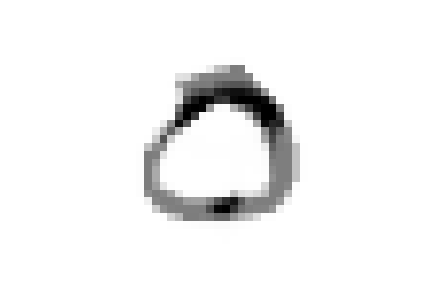
\includegraphics[width=0.14\textwidth]{figures/bary_wass_1_3.png}&

\includegraphics[width=0.14\textwidth]{figures/bary_wass_1_4.png}&
\multirow{3}{*}{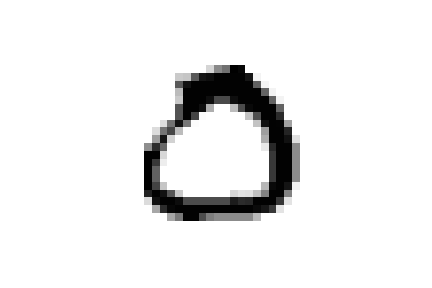
\includegraphics[width=0.14\textwidth]{figures/bary_l2_4.png}}
\\[-.15cm]
&

\includegraphics[width=0.14\textwidth]{figures/bary_wass_2_0.png}&

\includegraphics[width=0.14\textwidth]{figures/bary_wass_2_1.png}&

\includegraphics[width=0.14\textwidth]{figures/bary_wass_2_2.png}&

\includegraphics[width=0.14\textwidth]{figures/bary_wass_2_3.png}&
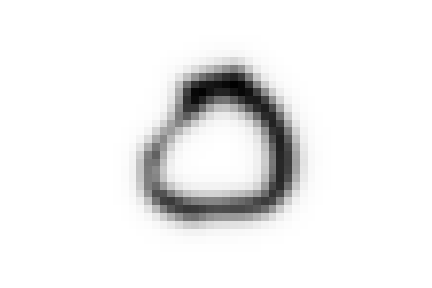
\includegraphics[width=0.14\textwidth]{figures/bary_wass_2_4.png}&

\\[-.15cm]
&

\includegraphics[width=0.14\textwidth]{figures/bary_GOT_0.png}&

\includegraphics[width=0.14\textwidth]{figures/bary_GOT_1.png}&

\includegraphics[width=0.14\textwidth]{figures/bary_GOT_2.png}&
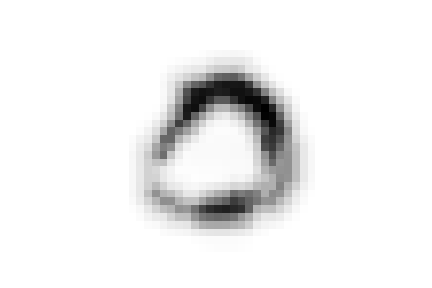
\includegraphics[width=0.14\textwidth]{figures/bary_GOT_3.png}&
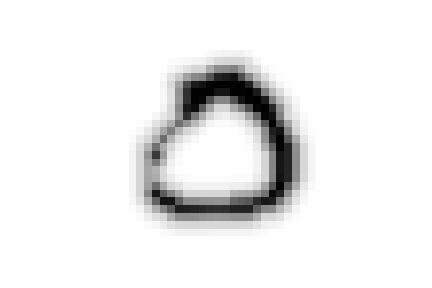
\includegraphics[width=0.14\textwidth]{figures/bary_GOT_4.png}&

\end{tabular}
\caption{The two first row starting from the above are Wasserstein barycenters using respectively square $\ell_2$ cost  and the cubic $\ell_3$ taken coordinate by coordinate. The last row represent the $\MOT$ barycenter with respect to these two costs. \textit{From left to right}:  Progressive barycentric transformation of ``$9$'' to ``$0$''. Both shapes are normalized to probability distributions.  \label{fig:bary90}}
\end{figure*}


\begin{figure*}[h]
\begin{tabular}{@{}c@{}c@{}c@{}c@{}c@{}c@{}c@{}c@{}}
\multirow{3}{*}{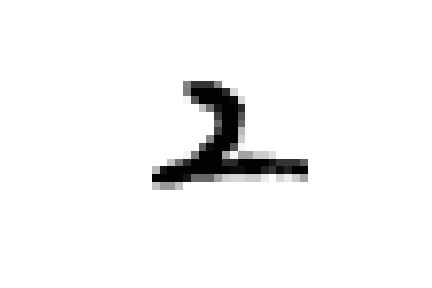
\includegraphics[width=0.14\textwidth]{figures/bary_l2_0_28.png}}&
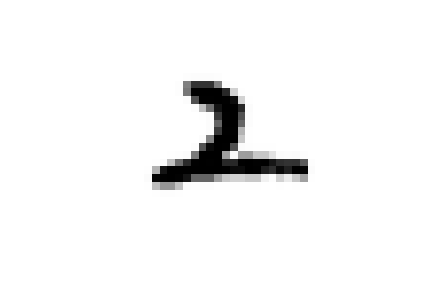
\includegraphics[width=0.14\textwidth]{figures/bary_wass_1_0_28.png}&
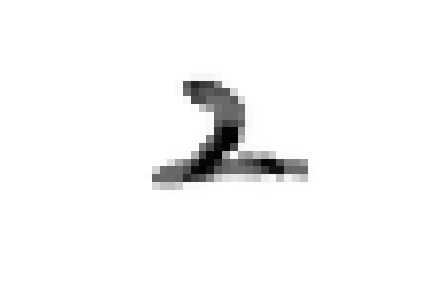
\includegraphics[width=0.14\textwidth]{figures/bary_wass_1_1_28.png}&

\includegraphics[width=0.14\textwidth]{figures/bary_wass_1_2_28.png}&
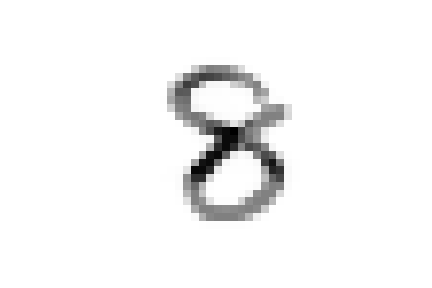
\includegraphics[width=0.14\textwidth]{figures/bary_wass_1_3_28.png}&
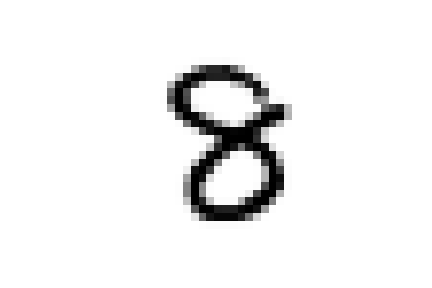
\includegraphics[width=0.14\textwidth]{figures/bary_wass_1_4_28.png}&
\multirow{3}{*}{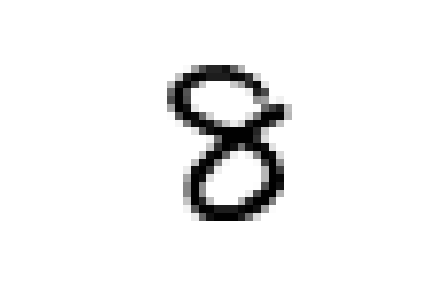
\includegraphics[width=0.14\textwidth]{figures/bary_l2_4_28.png}}
\\[-.15cm]
&
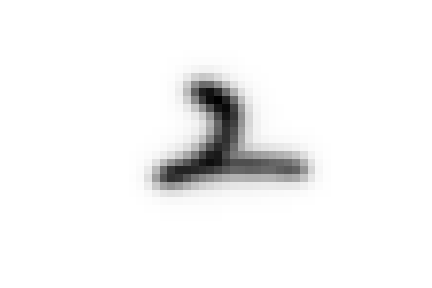
\includegraphics[width=0.14\textwidth]{figures/bary_wass_2_0_28.png}&
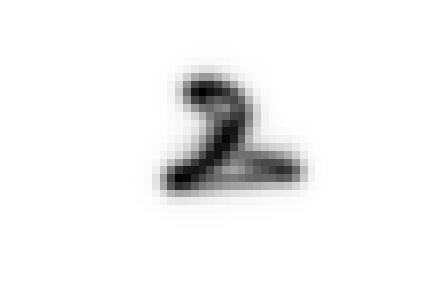
\includegraphics[width=0.14\textwidth]{figures/bary_wass_2_1_28.png}&
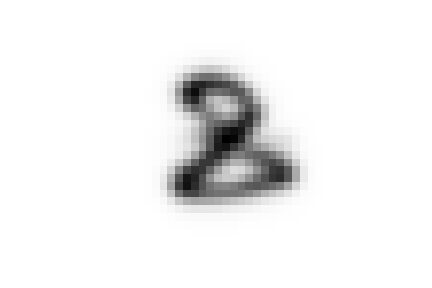
\includegraphics[width=0.14\textwidth]{figures/bary_wass_2_2_28.png}&
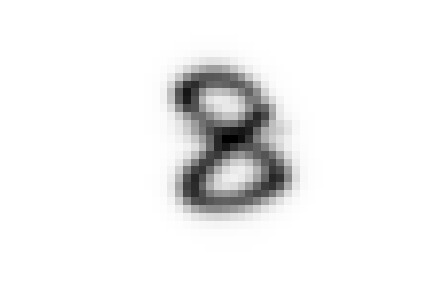
\includegraphics[width=0.14\textwidth]{figures/bary_wass_2_3_28.png}&
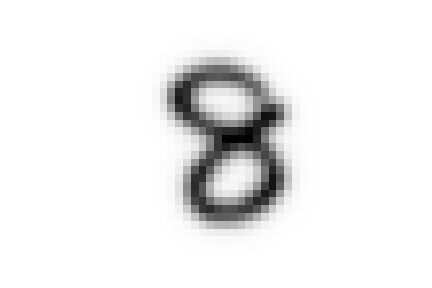
\includegraphics[width=0.14\textwidth]{figures/bary_wass_2_4_28.png}&

\\[-.15cm]
&
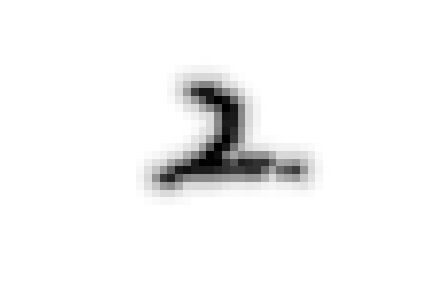
\includegraphics[width=0.14\textwidth]{figures/bary_GOT_0_28.png}&
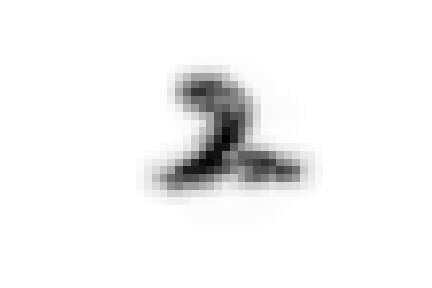
\includegraphics[width=0.14\textwidth]{figures/bary_GOT_1_28.png}&
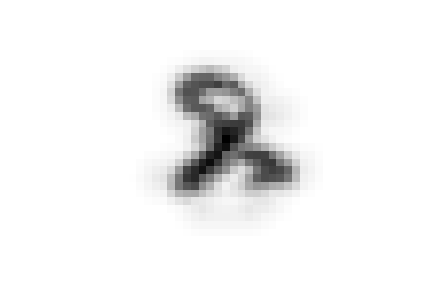
\includegraphics[width=0.14\textwidth]{figures/bary_GOT_2_28.png}&
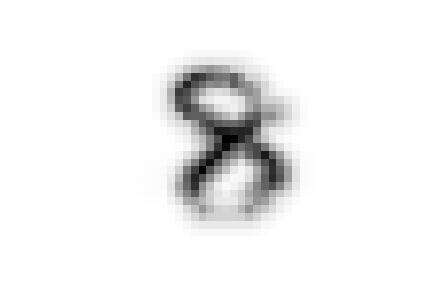
\includegraphics[width=0.14\textwidth]{figures/bary_GOT_3_28.png}&
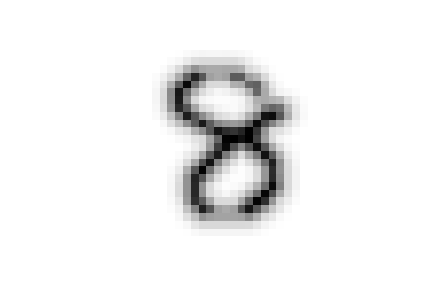
\includegraphics[width=0.14\textwidth]{figures/bary_GOT_4_28.png}&

\end{tabular}
\caption{The two first row starting from the above are Wasserstein barycenters using respectively square $\ell_2$ cost  and the cubic $\ell_3$ taken coordinate by coordinate. The last row represent the $\MOT$ barycenter with respect to these two costs. \textit{From left to right}:  Progressive barycentric transformation of ``$2$'' to ``$8$''. Both shapes are normalized to probability distributions.  \label{fig:bary28}}
\end{figure*}



\paragraph{Approximation for the Dudley Metric.} Figure~\ref{fig:result_acc} illlustrates the convergence of the entropic regularization approximation when $\epsilon\to 0$. To do so  we plot the relative error from the ground truth defined as $\text{RE}:= \frac{ \MOT_{\mathbf{c}}^{\bm{\varepsilon}}-\beta_d}{\beta_d}\ $ for different regularizations where $\beta_d$ is obtained by solving the exact linear program and $\MOT_{\mathbf{c}}^{\bm{\varepsilon}}$ is obtained by our proposed Alg.~\ref{algo:Proj-Sinkhorn}.

\begin{figure}[h!]
\centering
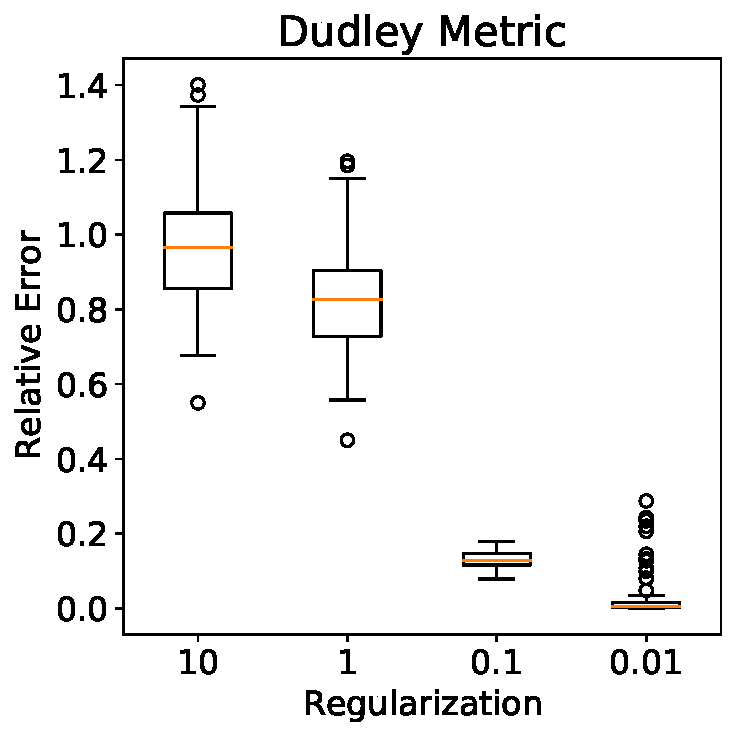
\includegraphics[width=0.6\linewidth]{figures/box_plot_accuracy.pdf}
\caption{In this experiment, we draw 100 samples from two normal distributions and we plot the relative error from ground truth for different regularizations. We consider the case where two costs are involved: $c_1= 2\times\mathbf{1}_{x\neq y}$, and $c_2=d$ where $d$ is the Euclidean distance. This case corresponds exactly to the Dudley metric (see Proposition~\ref{prop:GOT-holder}). We remark that as $\varepsilon\to 0$, the appproximation error goes also to $0$.\label{fig:result_acc}}
\end{figure}



\section{additional proofs (to include in main text)}

\todo{proof of optimality}
\begin{prv*}
Let $\mu$ and $\nu$ be two probability measures. Let $\mathbf{c}=(c_1,\dots,c_N)$ nonnegative lower semi-continuous costs. We have shown that the infimum defining $\MOT_\mathbf{c}(\mu,\nu)$ is attained. Let $\gamma^*$ be this infimum. Then at optimum we have shown that for all $i,j$, $\int c_id\gamma^*_i=\int c_jd\gamma^*_j = t$. Let denote for all $i$, $\mu_i=\Pi_{1\sharp}\gamma^*_i$ and $\nu_i=\Pi_{2\sharp}\gamma^*_i$. 

Let assume there exists $i$ such that $\int c_i d\gamma^*_i>\wass_{c_i}(\mu_i,\nu_i)$. Let $\gamma'_i$ realising the infimum of $\wass_{c_i}(\mu_i,\nu_i)$. Let $\epsilon>0$ be sufficiently small, then let define $\tilde{\gamma}$ as follows: for all $j\neq i$, $\tilde{\gamma}_j=(1-\epsilon)\gamma^*_j$. and $\tilde{\gamma}_i = \gamma'_i+\epsilon \sum_{j\neq i}\gamma^*_j$.
Then for all $j\neq i$, $\int c_j d \tilde{\gamma}_j = (1-\epsilon) t$ and $\int c_i d \tilde{\gamma}_i = \wass_{c_i}(\mu_i,\nu_i)+\epsilon \sum_{j\neq i} \int c_id\gamma^*_j$. It is clear that $\tilde{\gamma}\in \Gamma^N_{\mu,\nu}$. For $\epsilon>0$ sufficiently small, $\max_i\int c_id\tilde{\gamma}_i = (1-\epsilon) t<t$, which contradicts the optimality of $\gamma^*$.
\end{prv*}

\todo{proof of $W_{\min c}$ say we proved it in "generalized Fenchel duality}

\begin{proof}
\end{proof}
